%\documentclass[a4paper,twocolumn]{article}
\documentclass[a4paper,11pt]{book}

\usepackage[sort&compress,super]{natbib}
\usepackage[english]{babel}
\usepackage{amsmath, esint}
\usepackage{amssymb}
\usepackage{graphicx}
\usepackage{tabularx}                                 %% for tabulars with controllable width
\usepackage{caption}
\usepackage{subcaption}
%\usepackage{subfigure}                                %% for creating nested figures within figures
\usepackage{url}
\usepackage{array}
\usepackage{algorithm,algorithmic}
\usepackage{tikz}
\usepackage{url}  
\usetikzlibrary{arrows}
\usetikzlibrary{mindmap,trees}
\usepackage[overlay,absolute]{textpos}
%\usepackage[latin1]{inputenc}
\usepackage{wrapfig}
\usepackage{makeidx}
\usepackage{listings}
\usepackage{color}
\usepackage{xcolor}
\usepackage{enumitem}
\usepackage[normalem]{ulem}
\usepackage{mathtools}
\usepackage{lscape}
\usepackage{hyperref}
\usepackage[nameinlink]{cleveref}         %% Allows referencing subfigures. Must be loaded after hyperref

\DeclarePairedDelimiter{\ceil}{\lceil}{\rceil}
\DeclarePairedDelimiter{\floor}{\lfloor}{\rfloor}


% Rounded boxes functionality
\usepackage[framemethod=tikz]{mdframed}
\definecolor{mycolor}{rgb}{0.122, 0.435, 0.698}

\newmdenv[innerlinewidth=0.5pt, roundcorner=4pt,linecolor=mycolor, backgroundcolor=lightgray, innerleftmargin=4pt,
innerrightmargin=4pt,innertopmargin=2pt,innerbottommargin=2pt]{mybox}

%\usepackage[colorlinks,linkcolor=blue,anchorcolor=blue,citecolor=green]{hyperref} % hyper reference to contents 

%%%%%%%%%%%%%%%%%%%%%%%%%%%%%%%%%%%%%%%%%%%%%%%%%
%% Citation Shorthands
%%%%%%%%%%%%%%%%%%%%%%%%%%%%%%%%%%%%%%%%%%%%%%%%
\citestyle{plain}

\newcommand{\citeParMetis}{\cite{schloegel+2002, lasalle+2013}}
\newcommand{\citeGMSH}{\cite{geuzaine+2009}}
\newcommand{\citeGMSHCurv}{\cite{johnen+2012, toulorge+2013}}
\newcommand{\citeDune}{\cite{bastian+2008}}
\newcommand{\citeSuperLUDist}{\cite{li+2003}}











\makeindex



% The following parameters seem to provide a reasonable page setup.
\topmargin -1.0cm
\oddsidemargin 0cm
\evensidemargin 0cm
\textwidth 16.1cm 
\textheight 21cm
\footskip 1.0cm



\begin{document}

\lstset{language=C++, breaklines=true}



\begin{titlepage}




\begin{center}
    
\noindent \textsc{{\Large Dune-CurvilinearGrid}}

\vspace{5mm}

\noindent \textbf{\textsc{{\Large Parallel Dune Grid Manager for\\Unstructured Tetrahedral Curvilinear Meshes}}}
  
\vspace{2mm}
    
{\large
    
\noindent Aleksejs Fomins$^{\mathrm{a,b}}$ and Benedikt Oswald$^{\mathrm{b}}$

  }

\vspace{1mm}

\noindent $^{\mathrm{a}}$ Nanophotonics and Metrology Laboratory (\texttt{nam.epfl.ch})
\noindent Ecole Polytechnique F\'ederale de Lausanne (EPFL)
  
\vspace{1mm}

\noindent $^{\mathrm{b}}$ LSPR AG, Grubenstrasse 9, CH-8045 Z\"urich.
\noindent phone +41 43 366 90 74 - email: \texttt{aleksejs.fomins@lspr.ch} and \texttt{benedikt.oswald@lspr.ch}

\vspace{2mm}

%%\textbf{WEBSITE}

\end{center}











\pagebreak

%%%%%%%%%%%%%%%%%%%%%%%%%%%%%%%%%%%%%%%%%%%%%%%%%%%%%%%%%%%%%%%%%%%%%%%%
% BEGIN OF ABSTRACT
%%%%%%%%%%%%%%%%%%%%%%%%%%%%%%%%%%%%%%%%%%%%%%%%%%%%%%%%%%%%%%%%%%%%%%%%

\vfill

\noindent \textbf{\textsc{ABSTRACT}} - We introduce the \texttt{dune-curvilineargrid} module. The module provides the self-contained, parallel grid manager \texttt{dune-curvilineargrid}, as well as the underlying elementary curvilinear geometry class \texttt{dune-curvilineargeometry}. Both modules are developed as extension of \text{DUNE} \citeDune project, and conform to the corresponding standard interface. We expect the reader to be at least briefly familiar with the Dune interface to fully benefit from this paper.
%%
This work is carried out by a technology company LSPR AG. It is motivated by reliable and scalable design of nanooptical devices, performed by HADES3D family of electromagnetic codes. It is of primary scientific and industrial interest to model full 3D geometric designs as close to the real fabricated structures as possible. Curvilinear geometries improve both the accuracy of modeling smooth material boundaries, and the convergence rate of PDE solutions with increasing basis function order \cite{fahs2011}, reducing the computational effort required for robust modeling.
%%
\texttt{dune-curvilineargeometry} is capable to model simplex entities (edges, triangles and tetrahedrons) up to polynomial order 5 hard-coded, and up to arbitrary order via analytical procedures. Its most notable features are local-to-global and global-to-local coordinate maps, analytical and adaptive integration, explicit polynomial scalars, vectors and matrices (e.g. Jacobians and Integration Elements).
%%
\texttt{dune-curvilineargrid} module uses \texttt{dune-curvilineargeometry} to provide the following functionality: fully parallel input of curvilinear meshes in the \texttt{gmsh}\citeGMSH mesh format, processing only the corresponding part of the mesh on each available core; mesh partitioning at the reading stag (using \texttt{Parmetis} \citeParMetis); unique global indices for all mesh entities over all processes; ghost elements associated with the interprocessor boundaries; interprocessor communication of data for entities of the mesh of all codimensions via the standard \text{DUNE} data handle interface. There is also significant support for boundary integral codes, allowing arbitrary number of interior boundary surfaces, as well as parallel communication allowing for all-to-all dense coupling procedures.
%%
The \texttt{dune-curvilineargrid} grid manager is continuously developed and improved. Among other things, we are working on higher order basis functions for curvilinear grids, non-uniform adaptive h and p-refinement, periodicity. 
%%
As more work is being done on \texttt{dune-curvilineargrid}, this document will be updated. For the most recent version of the documentation, as well as for the source codes please refer to the following repositories: \\

\noindent
\url{http://www.github.com/lspr-ag/dune-curvilineargeometry}\\
\url{http://www.github.com/lspr-ag/dune-curvilineargrid}\\

\noindent
As well as our website\\

\noindent
\url{http://www.curvilinear-grid.org}




%%%%%%%%%%%%%%%%%%%%%%%%%%%%%%%%%%%%%%%%%%%%%%%%%%%%%%%%%%%%%%%%%%%%%%%%
% END OF ABSTRACT
%%%%%%%%%%%%%%%%%%%%%%%%%%%%%%%%%%%%%%%%%%%%%%%%%%%%%%%%%%%%%%%%%%%%%%%%

\end{titlepage}




%%%%%%%%%%%%%%%%%%%%%%%%%%%%%%%%%%%%%%%%%%%%%%%%%%%%%%%%%%%%%%%%%%%%%%%%
% ACKNOWLEDGEMENTS
%%%%%%%%%%%%%%%%%%%%%%%%%%%%%%%%%%%%%%%%%%%%%%%%%%%%%%%%%%%%%%%%%%%%%%%%


\pagebreak
\vspace{15mm}
\noindent \textbf{Acknowledgements} - While the architecture, implementation and down-to-earth programming work for \texttt{dune-curvilineargrid} grid manager is credited to Aleksejs Fomins and Benedikt Oswald, both authors are pleased to acknowledge the inspiration and support from the wider \text{DUNE} community. We mention names in alphabetical order and sometimes associated with a specific subject. In case we have forgotten to acknowledge an important contributor we kindly ask you to inform us and we will be happy to insert the name immediately. So, then, here we are:
%%
%%
\textit{Peter Bastian}, Professor at University of Heidelberg, Germany for initial suggestion to consider curvilinear tetrahedral grids in order to reduce the computational burden onto the complex linear solver;
%%
%%
\textit{Markus Blatt}, Heidelberg, Germany, based independent high performance computing and \text{DUNE} contractor, for numerous hints related to the build system and \text{DUNE} architecture;
%%
%%
\textit{Andreas Dedner}, professor, University of Warwick, United Kingdom, for numerous hints related to the \text{DUNE} architecture;
%%
%%
\textit{Jorrit 'Hippi Joe' Fahlke}, postdoctoral scientist, University of M\"unster, Germany, for numerous hints related to the \text{DUNE} architecture, grid API, grid testing and many other fields;
%%
%%
\textit{Dominic Kempf}, Phd student, University of Heidelberg, Germany for support w.r.t grid API implementation in \text{DUNE}, especially w.r.t \textit{CMake};
%%
%%
\textit{Robert Klo\"fkorn}, senior research scientist, IRISI, Norway, for support w.r.t grid API implementation in \text{DUNE};
%%
%%
\textit{Steffen Mu\"thing}, senior research scientist, IRISI, Norway, for support w.r.t grid API implementation in \text{DUNE};
%%
%%
\textit{Martin Nolte}, postdoctoral scientist, University of Freiburg im Breisgau, Germany, for numerous hints related to the \text{DUNE} architecture;
%%
%%
\textit{Oliver Sander}, professor, TU Aachen, Germany, for numerous hints related to the \text{DUNE} architecture, numerical integration and quadrature;




%%%%%%%%%%%%%%%%%%%%%%%%%%%%%%%%%%%%%%%%%%%%%%%%%%%%%%%%%%%%%%%%%%%%%%%%
% BY WHOM DEVELOPMENT WAS SPONSORED
%%%%%%%%%%%%%%%%%%%%%%%%%%%%%%%%%%%%%%%%%%%%%%%%%%%%%%%%%%%%%%%%%%%%%%%%

\vspace{20mm}
{\small
\noindent \textbf{LEGAL NOTICE} - The development of the \texttt{dune-curvilineargrid} grid manager is sponsored by a technology company \textbf{LSPR AG}, Grubenstrasse 9, CH-8045 Z\"urich, Switzerland. \textbf{LSPR AG} exclusively holds all rights associated with \texttt{dune-curvilineargrid}.
%%
The \texttt{dune-curvilineargrid} fully parallel grid manager will be made publicly available via \texttt{Github} and is a free software based on the GPLv2 license. Other licenses can be negotiated through \texttt{curvilinear-grid@lspr.swiss}.
%%
We herewith exclude any liability on the part of \textbf{LSPR AG} since the software is made available as is. Any user uses the software at his own risk and by no means \textbf{LSPR AG} assumes any responsibility for harmful consequences or any other damage caused by the use of the software. We emphasise that the whole project is governed by Swiss Law and nothing else. Especially, we reject any attempt of any other sovereign law to cover what we do.
}


\tableofcontents


\newpage
\chapter{Introduction}

%%%%%%%%%%%%%%%%%%%%%%%%%%%%%%%%%%%%%%%%%%%%%%%%%%%%%%%%%%%%%%%%%%%%%
% Curvilinear Grid Outline - Section on capabilities of the Grid
%%%%%%%%%%%%%%%%%%%%%%%%%%%%%%%%%%%%%%%%%%%%%%%%%%%%%%%%%%%%%%%%%%%%%

\section{Outline}
\subsection{Capabilities}

\noindent
Currently the curvilinear grid supports the following functionality.
\begin{itemize}
	\item Self-consistent grid manager supporting 3D tetrahedral curvilinear grids.
	\item GMSH input files of curvilinear orders 1-5. Usual linear geometries also supported
	\item Parallel mesh reader with scalability for large meshes and processors
	\item Mesh partitioning using ParMetis \textbf{CITE}
	\item Unique physical tag for each element and domain boundary. Read from GMSH file and accessible via grid methods.
	\item Unique global index for entities of all codimensions.
	\item Ghost elements of all codimensions (optional)
	\item Communication protocols for all codimensions
\end{itemize}

\noindent
The following functionality is currently NOT supported. As seen below, some of this functionality will be implemented in the nearest future, some other is not currently foreseen. We welcome contributions from the community
\begin{itemize}
	\item $[1-2 months]$ Location of containing element by global coordinate (via OCTree)
	\item $[1/2 year]$  Does NOT support global and local refinement
	\item $[1/2 year]$  Does NOT support hanging nodes
	\item $[1/2 year]$  Does NOT support periodic boundaries at the moment
	\item $[1 year]$    Does Not support curvilinear meshes of non-uniform order
	\item $[Undefined]$ Does NOT support 1D and 2D geometries. 
	\item $[Undefined]$ Does NOT support non-tetrahedral meshes.
	\item $[Undefined]$ Does NOT support front/overlap elements at the moment
\end{itemize}

\subsection{Design decisions}

\begin{itemize}
	\item User must provide globalId's for vertices and elements. [Automatically implemented by GMSH]
	\item User must provide all boundary segments inside GMSH file.
\end{itemize}


\subsection{Internal Structure}


Curvilinear Geometry:
\begin{itemize}
	\item Polynomial - Stores polynomials explicitly. Is able to perform basic arithmetic operations with polynomials, as well as differentiation and integration over a reference element.
	\item CurvilinearElementInterpolator
	\item CurvilinearGeometryHelper
	\item NumericalRecursiveInterpolationIntegrator
	\item CurvilinearGeometry
\end{itemize}

Curvilinear Grid
\begin{itemize}
	\item CurvilinearGMSHReader
	\item CurvilinearVTKWriter
	\item CurvilinearGridBase
		\subitem CurvilinearGridStorage
		\subitem CurvilinearGridConstructor
	\item CurvilinearGrid
	\item AllCommunicate
	\item VectorHelper	
	
\end{itemize}





\newpage
\chapter{Theory}

%%%%%%%%%%%%%%%%%%%%%%%%%%%%%%%%%%%%%%%
% Theory for Lagrange Polynomials
%%%%%%%%%%%%%%%%%%%%%%%%%%%%%%%%%%%%%%%
\subsection{Lagrange Polynomial Interpolation}
\label{theory-lagrange}

Below we present the theory of interpolation using \textit{Lagrange} polynomials, applied to simplex geometries, This section is inspired by \cite{koshiba+2000, ilic+2003, berrut+2004}, and is a summary of well-known results. The goal of \textit{Lagrange} interpolation is to construct a mapping $\vec{x} = \vec{p}(\vec{r})$ from local coordinates of an entity to global coordinates of the domain. In its own local coordinates, the entity will be denoted as a reference element \citeDune{}. A simplex reference element $\Delta_d$ of dimension $d$ is given by the following local coordinates:
%
\begin{table}[H]
\centering
\begin{tabular}{l l l}
\hline
  Label & Dimension & Coordinates \\ \hline
  $\Delta_0$ & 0 & $\{ 0 \}$ \\
  $\Delta_1$ & 1 & $\{ 0\}, \{ 1\}$ \\
  $\Delta_2$ & 2 & $\{ 0, 0 \}, \{ 1, 0 \}, \{ 0, 1 \}$ \\
  $\Delta_3$ & 3 & $\{ 0, 0, 0 \}, \{ 1, 0, 0 \}, \{ 0, 1, 0 \}, \{ 0, 0, 1 \}$
\end{tabular}
\caption{Reference element local coordinates}
\label{table:lagrange:refelement}
\end{table}
%
\noindent
Local simplex geometries can be parametrized using the local coordinate vector $\vec{r}$:
%
\begin{table}[H]
\centering
\begin{tabular}{l l l}
\hline
  Entity      & Parametrization    & Range \\ \hline
  Edge        & $\vec{r}=(u)$      & $u \in [0,1]$ \\
  Triangle    & $\vec{r}=(u,v)$    & $u \in [0,1]$ and $v \in [0, 1-u]$ \\
  Tetrahedron & $\vec{r}=(u,v,w)$  & $u \in [0,1]$, $v \in [0, 1-u]$ and $w \in [0, 1-u-v]$
\end{tabular}
\caption{Reference element parametrization in local coordinates}
\label{table:lagrange:parametrization}
\end{table}



%\paragraph{Interpolatory Vertices}
%\label{theory-lagrange-vertices}
\noindent
\textbf{Interpolatory Vertices}

\noindent
In order to define the curvilinear geometry, a set of global coordinates $\vec{x}_i = \vec{p}_i(\vec{r}_i)$, known as interpolatory vertices, is provided. By convention, the interpolatory vertices correspond to a sorted structured grid on a reference simplex, namely
\[\vec{r}_{i,j,k} = \frac{(k,j,i)}{Ord}, \;\;\; i=[0..Ord], \;\;\; j=[0..Ord-i], \;\;\; k=[0..Ord-i-j]\]
where $Ord$ is the interpolation order of the entity. It is useful to construct a bijective map from a structured local grid to the provided global coordinates. It is the job of the meshing software to ensure that the global geometry of an entity does is not self-intersecting, non-singular, and that its curvature is optimized for PDE convergence \cite{lenoir1986}. In general, a non-uniform local interpolatory grid should be used in order to minimize the effect of \textit{Runge} phenomenon \cite{runge1901}. It is not an issue for lower polynomial orders, and is the standard currently provided by the available meshing software, so we shall restrict our attention only to uniform interpolation grids. The number of interpolatory points on a uniform grid over the reference simplex is described by triangular/tetrahedral numbers \cref{table:lagrange:nvertex}. These numbers are conveniently also the numbers describing the total number $N_{Ord}$ of polynomially-complete monomials up to a given order:
%
\begin{table}[H]
\centering
\begin{tabular}{l l l l l l l}
\hline
  Entity \textbackslash Order & 1 & 2  & 3  & 4  & 5 & general \\ \hline
  Edge                        & 2 & 3  & 4  & 5  & 6 & $Ord+1$\\
  Triangle                    & 3 & 6  & 10 & 15 & 21 & $(Ord+1)(Ord+2)/2$\\
  Tetrahedron                 & 4 & 10 & 20 & 35 & 56 & $(Ord+1)(Ord+2)(Ord+3)/6$
\end{tabular}
\caption{Number of vertices in a uniform interpolatory grid over the reference simplex}
\label{table:lagrange:nvertex}
\end{table}





% \paragraph{Interpolatory Polynomials}
% \label{theory-lagrange-polynomials}
\noindent
\textbf{Interpolatory Polynomials}

\noindent
The number of interpolatory vertices $N_{Ord}$ given in \cref{table:lagrange:nvertex} exactly matches the total number of monomials necessary to construct a complete polynomial of order $Ord$ or less. It can be observed that the uniform simplex discretization exactly matches the binomial/trinomial simplex, also known as the Pascal's triangle, commonly used to visualize the complete monomial basis. We define the function $z^{(dim, i)}(\vec{u})$ as the set of all monomials of dimension $dim$ and order less than or equal to $i$. The first few sets for 1D, 2D and 3D are as follows:

\begin{table}[H]
\centering
\begin{tabular}{l l l}
\hline
  Edge & Triangle & Tetrahedron \\ \hline
  
  
  \begin{minipage}[l]{0.34 \textwidth}
  \begin{eqnarray*}
	z^{(1,1)}(u) &=& \{1, u\}, \\
	z^{(1,2)}(u) &=& \{1, u, u^2\}, \\
	z^{(1,3)}(u) &=& \{1, u, u^2, u^3\}, \\
	z^{(1,4)}(u) &=& \{1, u, u^2, u^3, u^4\}, \\
	z^{(1,5)}(u) &=& \{1, u, u^2, u^3, u^4, u^5\}, \\
	\mathrm{etc.} & &
  \end{eqnarray*}   
  \end{minipage} & 

  \begin{minipage}[l]{0.27 \textwidth}
  \begin{eqnarray*}
	z^{(2,1)}(u,v)	&=& \{1, u, v\}, \\
	z^{(2,2)}(u,v) &=& \{1, u, v, \\
	& & u^2, uv, v^2\}, \\
	\mathrm{etc.} & &
  \end{eqnarray*}
  \end{minipage} & 
  
  \begin{minipage}[l]{0.27 \textwidth}
  \begin{eqnarray*}
	z^{(3,1)}(u,v,w) &=& \{1, u, v, w\}, \\ 
	z^{(3,2)}(u,v,w) &=& \{1, u, v, w, \\
	& & u^2, uv, v^2, \\
	& & wu, wv, w^2\}, \\
	\mathrm{etc.} & &
  \end{eqnarray*}
  \end{minipage}
\end{tabular}
\caption{First few orders of the complete monomial basis for simplex entities }
\label{table:lagrange:monomial:function}
\end{table}

\noindent
The mapping $\vec{p}(\vec{r})$ is chosen to exactly fit all the interpolatory vertices $\vec{x}_i$. Since the numbers of interpolatory vertices and monomials is the same, the interpolatory vertices will have a \textit{unique} associated \textit{complete} polynomial basis. This is not the same for entities of other geometry types. For example, for hexahedra, the above numbers do not match. Therefore, one either has to use a structured local grid with incomplete polynomial order basis, or choose a more sophisticated local discretization. Volakis et al \cite{volakis+2006} adopt the former approach, interpolating a 9 node 2\textsuperscript{nd} order rectangle with 4\textsuperscript{th} order incomplete polynomial basis that has a convenient separable tensor product form. \\

\noindent
One way to formulate the local-to-global coordinate mapping is
\begin{equation}
	\vec{p}(\vec{r}) = \sum_j L_j(\vec{r})\vec{x}_j 
\end{equation}
\noindent
where $\vec{p}_j $ are the fixed interpolatory vertices, and $L_j$ are the \textit{Lagrange} polynomials, defined by their interpolatory property
\begin{equation}
	\label{equation-lagrangepol-interpolatory-property}
	L_j(\vec{r}_i) = \delta_{ij}
\end{equation}
\noindent
for all local interpolatory vertices $\vec{r}_i$. The advantage of this formulation is that the \textit{Lagrange} polynomials are independent of the interpolatory vertices $\vec{x}_i$, and thus can be pre-computed and reused for all entities of a given order. It remains to determine the exact form of \textit{Lagrange} polynomials. We will present a short proof that \cref{equation-lagrangepol-basis-link} holds
\begin{equation}
	\label{equation-lagrangepol-basis-link}
	z_i(\vec{r}) = \sum_j L_j(\vec{r}) z_i (\vec{r}_j) 
\end{equation}
\noindent
Here, $\{z\}$ is a vector of monomials as defined in \cref{table:lagrange:monomial:function}. Given a fixed dimension $dim$, \cref{equation-lagrangepol-basis-link} should hold for all polynomial orders $Ord$. Both sides of \cref{equation-lagrangepol-basis-link} are polynomials of order at most $Ord$, which means that they have at most $N_{Ord}$ free parameters. Therefore, to prove that \cref{equation-lagrangepol-basis-link} holds in general, it is sufficient to show that it holds for $N_{Ord}$ different arguments. Thus, it is enough to show that it holds for all $\vec{r} = \vec{r}_k$, which in turn is true due to \cref{equation-lagrangepol-interpolatory-property}. Finally, we can combine all monomials and \textit{Lagrange} polynomials into corresponding vectors
\begin{equation}
	\vec{z} (\vec{r}) = V \vec{L} (\vec{r})
\end{equation}
\noindent
where $V_{ij} = z_i (\vec{r}_j)$, and find the \textit{Lagrange} polynomial coefficients by solving the linear system
\begin{equation}
	\label{equation-lagrange-linear-system}
	\vec{L} (\vec{r}) = V^{-1} \vec{z} (\vec{r})
\end{equation}

\noindent
It is important to note that the resulting interpolated geometry in global coordinates is not completely defined by the shape of its boundary, as the entire volume of the geometry inside the entity undergoes this polynomial transformation. \\


% \paragraph{Implementation for Simplices}
% \label{subsection-simplexgrid}
\noindent
\textbf{Implementation for Simplices}

\noindent
In this section we discuss how to efficiently enumerate the simplex interpolatory points and to construct the reference simplex grid. \\

\noindent
Let us define a simplex $\Delta^{\dim}_{n}$ of integer side length $n$, and place a set of points $\vec{\eta} \in \mathbb{Z}^{\dim}$ at unit intervals. This can be done by using nested loops
\begin{itemize}
	\item $\Delta^{1}_n = \{(i)\}$, for $i = [1$ to $n]$
	\item $\Delta^{2}_n = \{(j,i)\}$, for $i = [1$ to $n]$, $j = [1$ to $n - i]$
	\item $\Delta^{3}_n = \{(k,j,i)\}$, for $i = [1$ to $n]$, $j = [1$ to $n - i]$, $k = [1$ to $n - i - j]$
\end{itemize}

\noindent
Then, each integer vertex $(\Delta^{d}_n)_i$ corresponds exactly to the power of $u,v,w$ in the expansion of
\[ (1 + u)^n = \sum_{i=0}^n C^{(\Delta^{1}_n)_i}_n u^{(\Delta^{1}_n)_{i,1}} \]
\[ (1 + u + v)^n = \sum_{i=0}^n C^{(\Delta^{1}_n)_i}_n u^{(\Delta^{1}_n)_{i,1}} v^{(\Delta^{1}_n)_{i,2}} \]
\[ (1 + u + v + w)^n = \sum_{i=0}^n C^{(\Delta^{1}_n)_i}_n u^{(\Delta^{1}_n)_{i,1}} v^{(\Delta^{1}_n)_{i,2}} w^{(\Delta^{1}_n)_{i,3}} \]

\noindent
where $C^{i}_n, C^{i,j}_n$ and $C^{i,j,k}_n$ are the binomial, trinomial and quatrinomial coefficients. The powers of the parameters given in the above expansion correspond to the complete monomial basis for a polynomial of order $d$. The local coordinates of the uniform grid over the reference simplex can then be written as $r_i = \frac{1}{n}(\Delta^{d}_n)_i$ (see \cref{fig:lagrange:enumerationconstruction})

\begin{figure}[hp]
    \centering
    
\includegraphics[scale=2.0]{images/curvilinear-numbering-generation}
    \caption{Construction of the uniform grid interpolatory points (right) from the \textit{Cartesian} coordinate enumeration}
    \label{fig:lagrange:enumerationconstruction}
\end{figure}

\noindent
After the monomials and the parametric interpolation points have been constructed, it remains to construct the interpolation matrix $V$ by evaluating the monomials at the interpolation points and to solve the linear system \cref{equation-lagrange-linear-system}, obtaining the \textit{Lagrange} polynomials. This has been implemented both explicitly, calculating and hard-coding all the simplex \textit{Lagrange} interpolatory polynomials, and implicitly, implementing symbolic polynomial arithmetic. The latter has the advantage of unrestricted polynomial order, as well as the freedom of further analytic manipulation using of symbolic arithmetic and explicit differential operators, but comes at the cost of slight computational overhead. \\

\noindent
The optimization of \textit{Lagrange} polynomial evaluation is of crucial importance, since they are typically evaluated a significant amount of times, especially during the integration and minimization procedures. Our implementation of \textit{Lagrange} polynomials benefits from the following observations:
\begin{itemize}
  \item Each \textit{Lagrange} polynomial of a given order uses the same monomial summands. It is thus of an advantage to evaluate all the \textit{Lagrange} polynomials at the same time, first evaluating all the necessary monomials, and then re-using the evaluated monomials to compute the polynomials.
  \item Along the same lines, evaluating all monomials of a given order at the same time is cheaper than evaluating them separately. Lower order monomials can be used to construct higher order monomials by doing a single multiplication per monomial.
\end{itemize}








%%%%%%%%%%%%%%%%%%%%%%%%%%%%%%%%%%%%%%%
% Theory for global and local mappings
%%%%%%%%%%%%%%%%%%%%%%%%%%%%%%%%%%%%%%%
\subsection{Coordinate transformation}
\label{sec:theory:coordinatetransform}

In order to calculate the coordinate transformation properties, one requires the knowledge of the local-to-global map $\vec{p}(\vec{r})$ and its first partial derivatives. Currently, \curvgeom{} only provides \textit{Lagrange} polynomials themselves as hard-coded expressions. Their derivatives are not yet available as hard-coded quantities, and thus are constructed by differentiating the symbolic polynomial map. This is, naturally, a little slower than having hard-coded derivatives. The advantage of analytical formulation is that the user can further apply algebraic and differential operators to the symbolic map to obtain, for example, a \textit{Hessian} matrix of the transformation.  \\

\noindent
\textbf{Local-to-Global map}
%
Local-to-global map $\vec{p}(\vec{r})$ is computed numerically using hard-coded \textit{Lagrange} polynomials when the order is below or equal to 5, and through analytic procedures otherwise. \\

\noindent
\textbf{\textit{Jacobian} and Inverse \textit{Jacobian}}
%
The local-to-global mapping is represented by a vector of symbolic polynomials, further computing \textit{Jacobian} matrix $J_{ij}(\vec{r}_0) = \partial_{r_i} p_j (\vec{R}) |_{\vec{r}_0}$ using exact partial differentiation provided by the polynomial class. This results in a matrix of polynomials, which can be evaluated for the desired local coordinates. The \textit{Jacobian} inverse and the integration element are then computed numerically using the \dune{} provided linear algebra routines, the matrix inverse $J^{-1}$ and pseudo-determinant $dI = \sqrt{\det(JJ^T)}$ respectively (see \cref{appendix:integrationelements:proof}). \\

\noindent
\textbf{Global-to-Local map}
%
For polynomial elements, global-to-local map is the inverse of a polynomial map. Given the matching world and entity dimension, the method searches for the exact coordinate local to the element, that corresponds to the provided coordinate. Further, this method is extended to elements with $(dim_{elem} \leq dim_{world})$ by converting it to an optimization problem
\begin{equation}
  \label{eq-theory-mapping-optimization}
  \vec{r} : |\vec{p}(\vec{r}) - \vec{x} |^2 \rightarrow \min
\end{equation} 
searching for the local coordinate closest to the inverse of the desired global coordinate in terms of distance in global coordinates. \\

\noindent
While this problem is always uniquely solvable in linear case, in the curvilinear case it poses several additional challenges
\begin{itemize}
	\item The polynomial interpolatory map $\vec{p}(\vec{r})$ is strictly bijective inside the reference element, which must be ensured by the mesh generator. However, this need not be the case outside it. For example, $p(r) = r^2$ is a bijective 1D local-to-global map for an edge defined on $[0,1]$. However, the map is clearly non-invertible for all $p(r) \leq 0$, and thus asking for a local coordinate corresponding to the global coordinate $-1$ has no defined answer.
	\item Curvilinear geometries have singularities, e.g. $r = 0$ in the previous example. At these points the integration element is zero, which most simple iterative methods can not handle. It is expected that the meshing software provides curvilinear entities with non-singular geometries, since this would result in infinitesimal global volumes associated with finite local volumes, destabilizing optimization methods and integration routines. There is no restriction on the singularity being in the near vicinity of the element, which may be enough to significantly damage convergence.
	\item For $(dim_{elem} \leq dim_{world})$, the optimization problem given by \cref{eq-theory-mapping-optimization} is highly nonlinear. There may be multiple solutions, even uncountably many.
\end{itemize}

\noindent
For obvious reasons we will not solve the problem directly, as searching for the roots of a system of polynomial equations in 2D and 3D is well-known to be a challenging task \cite{canny+1989}. Instead, the problem is solved by a first order \textit{Gauss-Newton} method \cite{bjoerck+1996}, extending the implementation from \texttt{dune-multilineargeometry}.

\noindent
Based on an exchange with the \dune{} user community, we have realised that in order to satisfy all use cases we need to implement two distinct methods
\begin{itemize}
  \item Restrictive method, useful to those who want to find the element containing the global coordinate, as well as the local coordinate inside that element. If the provided global coordinate is inside the element, the method will return a success and a valid local coordinate. Otherwise, the method will return a fail and no coordinate at all, meaning that the global coordinate is not inside the element. This method also extends to lower dimension entities, finding the local coordinate within the element (!), which minimizes the distance to the provided global coordinate. Given a well-defined map (non-singular in the vicinity of the element), this method is guaranteed to converge.
  \item Non-restrictive method, useful to those who wish to extrapolate the global-to-local map beyond the reference element. This method searches for the inverse (or the distance minimizer) over the entire local domain. This is a best effort method - due to the above mentioned difficulties, it is expected to fail to converge for some maps and global coordinates. In this case, an exception is thrown.
\end{itemize}

\noindent
Below we outline the algorithm of the restrictive method:

\begin{mybox}
\begin{enumerate}
	\item Let $\vec{x}_0$ be the requested global coordinate
	\item Start with a local point $\vec{r}_0$ guaranteed to be inside the element (e.g. its center),
	\item Iteratively choose better approximations for local coordinate using \[\vec{r}_{n+1} = \vec{r}_n + \vec{d}(\vec{r}_n)\] where $\vec{d}(\vec{r}_n)$ is the least squares solution of
	        \[ J(\vec{r}_n) \vec{d}(\vec{r}_n) = \vec{p}(\vec{r}_n) \] and $J(\vec{r})$ is the \textit{Jacobian} matrix.
	\item The iterative process is finished when the global coordinate distance converges to a given tolerance level $\epsilon$ in terms of the two-norm
	        \[ \epsilon_n = |\vec{p}(\vec{r}_n) - \vec{x}_0 |^2 \leq \epsilon \]
	\item The iteration is terminated prematurely if there is enough evidence that the optimal vertex is outside the element. For this, two criteria are used: the running estimate being far outside the element \[|\vec{p}_0 - \vec{p}_i|_2 > 4 R_{elem}\] and the convergence speed being significantly slower than quadratic.
\end{enumerate}
\end{mybox}

\noindent
We are still looking to improve this method. It correctly predicts the global coordinates being inside and outside the element for most of our tests, but fails to identify the boundary points inside the element for certain cases.


%%%%%%%%%%%%%%%%%%%%%%%%%%%%%%%%%%%%%%%
% Theory for integration over curvilinear entities
%%%%%%%%%%%%%%%%%%%%%%%%%%%%%%%%%%%%%%%
\section{Integration}
\label{sec:theory:integration}

An important method of any entity is calculating scalar and vector parametric integrals over its global volume, the simplest being the volume itself. In general form the integral can be written as
\[ \int f(\vec{x}) d^{\dim} x = \int f(\vec{r}) \mu(\vec{r}) d^{\dim} r \]
where $\vec{x}$ and $\vec{r}$ are global and local coordinates respectively, $f(\vec{x})$ some function defined over the element, and the function $\mu(\vec{r})$ associated with the change of coordinates, called the integration element. In the original \textit{dune-geometry} paradigm, geometry class itself does not perform any integration, but calculates the integration element$\mu(\vec{r})$. Later, the user performs the integration over the reference element by using, for example, one of the quadrature rules\cite{abramowitz+1970} provided by \textit{dune-geometry}. A standard numerical quadrature can written as a weighted sum
\[ \int f(\vec{r}) \mu(\vec{r}) d^{\dim} r = \sum_i f(\vec{r}_i) \mu(\vec{r}_i) w_i  \]
where the $r_i$ and $w_i$ are the quadrature points and weights. The sampling points and weights are a property of the quadrature rule used, and can be reused for all integrands given fixed local geometry and approximation order. More precisely, given a polynomial order $p$, one can construct a finite numerical quadrature, which will be exact for polynomials of order $p$ and below, and thus well approximate integral over any function, that is well-approximated by a polynomial. \\

\noindent
Numerical quadrature methods in practice are considerably faster than any other known method for geometry dimensions $\dim \leq 3$ \cite{schurer2003}, but they also have disadvantages. Firstly, they are inaccurate for functions that can't be approximated by reasonable order polynomials. Secondly, numerical quadratures for non-trivial domains (e.g. simplices) have so far only been calculated only to very moderate orders (~20) \cite{zhang+2008}. Finding a numerical quadrature is equivalent to finding roots of a polynomial, which is extremely hard in more than 1 dimension. One way to overcome these difficulties is to transform the integration domain to a cuboid using a Duffy transform (for full derivation, see abstract \ref{section-abstract-duffy-transform})

\[ \int_0^1 \int_0^{1-x} f(x,y) dx dy = \int_0^1 \int_0^1 f(x, (1-x)t ) dx dt  \]

\noindent
The advantage of the cuboid geometry is that a quadrature rule can be constructed from a tensor product of 1D quadratures, which are readily available at relatively high orders. Quadrature rules created in this way have more points per order than the optimal rules, created specifically for the desired (e.g. simplex) geometries. Nevertheless, they work, and are availabe in, e.g., \textit{dune-geometry} up to order 61. We are aware of existence of advanced methods to improve performance of quadrature integration (e.g. Sparse Grids \cite{petras2000}), but they are beyond the scope of this paper. \\

%%%\subsection{Overview of available numerical methods}
%%%
%%%\noindent
%%%Below is presented a short summary of integration method types known to us: \\
%%%
%%%\noindent
%%%\textbf{Gaussian Quadrature}: The method available in DUNE.
%%%\begin{itemize}
%%%	\item This method calculates the integral as a linear product of the integrand $f(\vec{r})$ values at specific precomputed points $\vec{r}_i$ with specific precomputed weights $w_i$, namely $I = \sum_i w_i f(\vec{r}_i)$. Thus the main advantage of this method is its computational cost, which is small for low order polynomial integrands.
%%%	\item Optimal quadrature points are only available for small dimensions. Finding such point sets for high dimension polynomials is very involved and is known to suffer from finite precision of floating point arithmetic. Alternatively, a suboptimal point distribution can be obtained from a tensor product space of 1D point distributions, whose size grows exponentially with integration dimension.
%%%	\item Gaussian Quadrature is constructed with the idea of calculating exact integrals for integrands being polynomial up to a given order. However, when integrating over a curved boundary, thte integration elemen is a square root of a polynomial, and polynomials really badly approximate square root, especially for small arguments, which can easily happen for highly curved elements. Not to mention that one, in principle, could with to integrate arbitrary (within reason) functions over the element. Thus
%%%		\subitem - Can GQ estimate integration error for non-polynomial functions?
%%%		\subitem - Can it be made hierarchical to have control over error by refinement?
%%%		\subitem - What would be the convergence rate to compare with other methods?
%%%\end{itemize}
%%%
%%%\noindent
%%%\textbf{Interpolatory adaptive refinement}: The method currently implemented in LagrangeGeometry subclass
%%%\begin{itemize}
%%%	\item - Evaluates integral over element, approximating the integrand by an interpolatory polymomials of two hierarchical orders (2 and 4 at the moment) \textbf{[IMAGE HERE]}
%%%	\item - The running integration error is approximated by the difference between the analytical integrals calculated from these two interpolatory polynomials.
%%%	\item - The higher order element is split into into sub-elements of lower order, and the integration proceeds recursively.
%%%	\item - Every time an element is split, its previous running error is subtracted from the total error, and the running errors of the sub-elements are added to the total error. Thus, the integration is terminated when total approximated error is below selected tolerance. 	
%%%		\subitem - using heap structure ordered by the approximate error of the element. This way avoids recursion, and at every iteration selects the element which has worst error, then refines it.
%%%		\subitem - When splitting, the previously calculated points are not re-calculated but hierarchically re-used by sub-elements. The sub-element only needs to be refined to a higher hierarchical order, by adding more points.
%%%	\item \textit{Possible improvement - Performance}. As the the refined element does not check if the neighboring elements are also being refined, so they both sample on the boundary twice. Does there exist a method to store/find intersection refinements faster than just compute 2nd time. Using order 4 for every new refined triangle we sample 9 new points, out of which 2 are being wasted, thus $22\%$ inefficient.
%%%\end{itemize}
%%%
%%%\noindent
%%%\textbf{Monte-Carlo integration} - according to above mentioned paper, good for dimensions 7 and above.
%%%\begin{itemize}
%%%	\item Randomly samples function over element, integral is approximated by the average over the sample
%%%	\item natural error estimate using sample standard deviation
%%%	\item Stratified Sampling: if after a set number of iterations sample error is larger than expected, then function is highly non-uniform. Split element in equal parts and continue recursively.
%%%	\item Markov Chain Monte Carlo (MCMC): Uses random walk to sample the integrand, thus concentrating the sample points where the function varies most. Can use Metropolis-Hastings to also adapt the sampling distribution.
%%%\end{itemize}
%%%
%%%\noindent
%%%\textbf{Interpolatory Spline integration} - this is just another idea...
%%%\begin{itemize}
%%%	\item Makes grid over element, cubic-interpolates all consecutive partially-overlapping segments, integrates analytically over each segment.
%%%		\subitem -tricky part 1: when interpolatory segments intersect, with what weights to take the intersecting parts
%%%		\subitem -tricky part 2: how well does this method interpolate boundaries of the element (being close to edges and faces)
%%%		\subitem -tricky part 3: how to estimate error of integration and necessary grid step?
%%%		\subitem - Any way to do the refinement or error-control?
%%%\end{itemize}

The integration in \textit{dune-curvilineargeometry} focuses on two additional questions:
\begin{itemize}
	\item Integrating polynomials of arbitrary order
	\item Integrating smooth functions with no a priori knowledge of the optimal polynomial approximation order.
\end{itemize}

\noindent
\subsection{Analytic Integration}
To address the first question, \textit{dune-curvilineargeometry} implements a polynomial class, which is stored as a sum of monomials of a given order. Integrals over monomials of any given order can be expressed analytically \cref{appendix-proof-simplexintegral}, and thus an analytical integral over arbitrary polynomial is given by the sum of such monomial integrals \\

\begin{table}[h]
\centering
\begin{tabular}{l | l}
\hline
Cuboid Integrals &
\begin{tabular}{@{}c@{}}
$ \int_0^1 x^i dx = \frac{1}{i+1} $ \\
$ \int_0^1 \int_0^1 x^i y^j dx dy = \frac{1}{(i+1)(j+1)} $ \\
$ \int_0^1 \int_0^1 \int_0^1 x^i y^j z^k dx dy dz = \frac{1}{(i+1)(j+1)(k+1)} $ \\
\end{tabular} \\ \hline
Simplex Integrals &
\begin{tabular}{@{}c@{}}
$ \int_0^1 x^i dx = \frac{1}{i+1} $ \\
$ \int_0^1 \int_0^{1-x} x^i y^j dx dy = \frac{i! j!}{(i + j + 2)!} $ \\
$ \int_0^1 \int_0^{1-x} \int_0^{1-x-y} x^i y^j z^k dx dy dz = \frac{i! j! k!}{(i + j + k + 3)!} $ \\
\end{tabular} \\
\end{tabular} \\
\end{table}

\noindent
The polynomial class implemented in \textit{dune-curvilineargeometry} provides a method that implements analytical integration. \\

\noindent
\subsection{Adaptive Integration}
In its general form, a scalar integral over an element can be written as \[\int f(\vec{r}) d^{\dim} x = \int f(\vec{r}) \mu(\vec{r}) d^{\dim} r,\] where the integration element is given by \[\mu(\vec{r}) = \sqrt{\det(J J^T)},\] and $J$ is the Jacobian matrix. \\

\noindent
In the case of matching element and space dimension (like volume in 3D, or area in 2D), the integration element simplifies to $|\det J|$. Even though absolute value is not a polynomial function, it can be observed that $\det J$ is not allowed to change sign over the element, as that would result in self-intersection. Also the case of $\det J = 0$ should be avoided by meshing tool, as it leads to zero volumes in global coordinates. It remains to evaluate the integration element it anywhere inside the element and discard the minus sign if it happens to be negative. Then, if the integrand is well-approximated by a polynomial, so is the entire integral, and thus it can be integrated exactly. \\

\noindent
In the case of mismatching dimensions (like area in 3D, or length in 2D and 3D), the expression for $\mu(\vec{r})$ cannot be simplified, as it is a square root a polynomial that itself is not a square of another. Such integrals, in general, do not possess a closed form solution and have to be dome numerically. To tackle this problem, \textit{dune-curvilineargeometry} provides a recursive integrator class, which iteratively increases the quadrature order until the estimated integration error converges to a desired tolerance level. This method can take several seconds for surface area calculation of near-singular geometries requiring very high polynomial order, but on average it converges much faster. The method accepts integrands in terms of functors overloading a skeleton class, and the \textit{dune-curvilineargeometry} uses it internally to provide volumes and surfaces of curvilinear entities, only requiring the user to additionally specify the desired tolerance level. \\

\noindent
In addition, the integrator class supports simultaneous integration of vector and matrix integrands via $Dune::DynamicVector$ and $Dune::DynamicMatrix$, as well as $std::vector$. The motivation of this implementation is due to the fact that frequently simultaneous evaluation of a vector or a matrix is considerably cheaper than individual evaluation of each component. The method provides several possible matrix and vector convergence error estimates (such as 1 and 2-norm), which can be freely selected to adapt to the problem at hand.\\

\noindent
Still, there is definitely room for improvement. According to \cite{schurer2003}, best results in low-dimensional numerical integration are achieved by adaptive quadrature of high degree, whereas Monte-Carlo methods perform better for high-dimensional integrals. Thus, using an external adaptive library, for example the GSL extension due to Steven G. Johnson (\url{http://ab-initio.mit.edu/wiki/index.php/Cubature}) could be of definite advantage. This library is based on Clenshaw-Curtis quadrature, which has the advantage of being hierarchical. Thus, it can be refined to iteratively improve precision by re-using the points already calculated for lower order integrals. Another speedup could be provided by employing sparse grids \cite{petras2000} \\

%%%\subsection{Integration Element - Vector}
%%%
%%%When integrating vector functions we are mostly interested in the integrals over boundary surfaces and edges, namely $\int_{\partial V} \vec{f}(\vec{r}) \cdot \vec{n}(\vec{r}) d(\partial V)$. For an edge in 2D the following expression for the tangential and normal integration elements (up to a sign convention) can be found:
%%%\[ d\vec{l}_{\parallel} = (\partial_u p_x, \partial_u p_y)du \; \; \; \; \; d\vec{l}_{\perp} = (\partial_u p_y, -\partial_u p_x)du  \]
%%%
%%%\noindent
%%%For a vector in 3D the tangential integration element is not defined, but the normal integration element is
%%%\[ d\vec{S} = (\partial_u \vec{p} \times \partial_v \vec{p})du \; dv  \]
%%%
%%%\noindent
%%%Thus, given polynomial vector basis functions $\vec{f}$ and polynomial interpolation, the scalar (and, if necessary, vector) products $\vec{f}(u) \cdot d\vec{l}(u)$ and $\vec{f}(u,v) \cdot d\vec{S}(u,v)$ are also polynomial, and can be integrated exactly using analytic polynomial integration code.



%%%%%%%%%%%%%%%%%%%%%%%%%%%%%%%%%%%%%%%
% Theory for point location (OCTree)
%%%%%%%%%%%%%%%%%%%%%%%%%%%%%%%%%%%%%%%
%%\section{OCTree}
\label{theory-octree}

\subsection{Point location with respect to a plane}

Assume that a plane is given by 3 coordinates $\vec{a}, \vec{b}, \vec{c}$, and we would like to check on which side of this plane the point $\vec{p}$ is. This is uniquely given by a function
\begin{equation}
\label{equation-point-plane-test}
	ptest(\vec{a}, \vec{b}, \vec{c}, \vec{p}) = \mathrm{sgn} \{ \det (\vec{a} - \vec{p}, \vec{b} - \vec{p}, \vec{c} - \vec{p}) \}
\end{equation}
\noindent
This function takes values $1,-1$ for corresponding sides of the plane, and $0$ if the point is on the plane.

\subsection{Locating the element the given global coordinate belongs to}
\label{subsection-locating-element}

\noindent
Current convention: loop over all elements in the mesh, check if the point is inside the element using the method below. \\


\noindent
This method has $O(1)$ initialization cost, but $O(N) * ins$ query cost, which becomes wastefully slow as the number of points to locate grows. Here $ins$ is the cost of $is\_inside$ method, which has constant complexity if the query point is far away from the triangle, but requires an iterative method for nearby methods.

\noindent
There are two ways one can implement the above idea: \\
\textbf{First method:}
\begin{enumerate}
	\item Iterate over all elements, use linear $check\_inside()$
	\item For the element for which linear $check\_inside() = true$ run the nonlinear $check\_inside()$
	\item If the nonlinear $check\_inside() = false$, recursively do nonlinear $check\_inside()$ on the neighbors of the element.
\end{enumerate}
\textbf{Second method:}
\begin{enumerate}
	\item Iterate over all elements, use nonlinear $check\_inside()$
\end{enumerate}
\noindent
The first method is better, because it will on average have less runs of the iterative method, as if the point is located in a linear element, it has high probability of being located inside the nonlinear element with the same corners. \\

\noindent
An improvement would be to implement an OCTree, which will have a recursively-refined cubic mesh over the tetrahedral one, and upon initialization would place each of the tetrahedrons recursively within one or more leafs of the tree. Thus the initialization cost would be $O(N \log(N))$, and the cost of a single query $O(\log(N)) + M * inc$, where $M$ is the number of neighbors an element has. This is a considerable improvement for large number of queries. \\

\noindent
\textbf{OCTree method}:
\begin{enumerate}
	\item Construct the OCTree - grid the domain, build the hierarchical tree, place the correct element labels into each leaf
	\item For each query, locate the leaf the query point corresponds to
	\item Proceed by using one of the above methods on the element set of the leaf
\end{enumerate}

\begin{figure}[hp]
    \centering
    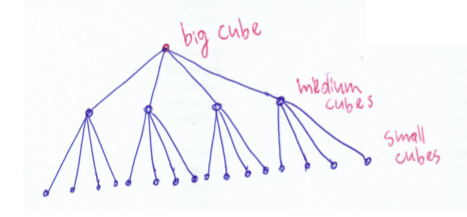
\includegraphics[scale=0.7]{doc-pics/pic-octree-3.png}
	\caption{OcTree internal structure}    
    
    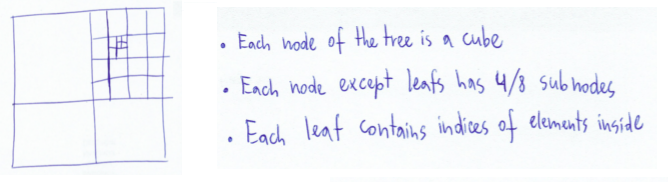
\includegraphics[scale=0.7]{doc-pics/pic-octree-1.png}
	\caption{OcTree grid}    
	
    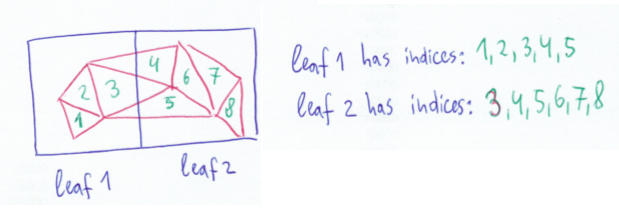
\includegraphics[scale=0.7]{doc-pics/pic-octree-2.png}
	\caption{OcTree partition of elements}    
    %\caption{Awesome Image}
    %\label{fig:awesome_image}
\end{figure}


\noindent
How does this work with parallel processing?

\subsection{Checking if a global coordinate is inside a given element (straight sided)}
\label{subsection-isinside-linear}

\noindent
For straight-sided elements the conversion between global and local coordinates is 1-to-1 in the whole space.
Therefore, it is sufficient to find the corresponding local coordinate and use the $referenceelement$ method $checkInside$. \\

\noindent
For example, for a simplex the $is\_inside(u,v,w)$ for local coordinates $(u,v,w)$ looks like 
\[u \geq 0\ \&\ v \geq 0\ \&\ w \geq 0,\ \&\ u+v+w \leq 0. \]

\noindent
Naturally, the global-local map has a finite precision, therefore the $checkInside$ method corrects for that by having a small tolerance for above inequalities, thus avoiding the case where a boundary point would be considered outside both neighboring elements because of numerical errors.


\subsection{Checking if a global coordinate is inside a given element (curvilinear elements)}
\label{subsection-isinside-nonlinear}

\noindent
This method is only defined if ($(dim_{elem} = dim_{world})$). For discussion see the $local()$ method discussion.

\noindent
In principle, this method requires an iterative solver, but first we run two simpler tests which immediately identify some of the points inside or outside of the element. \\

\noindent
\textbf{Far-point test}:
\begin{enumerate}
	\item Define linear center $\vec{p}_{CoM}$ of an element as the center of mass of its corners.
	\item Define the radius of an element $R$ as the largest distance between $\vec{p}_{CoM}$ and a point $\vec{p}_b$ on its boundary
	\item Define linear radius $R_{lin}$ to be the largest distance between $\vec{p}_{CoM}$ and one of the corners of the element. It can be shown that $R_{lin} = \frac{\sqrt{dim^2 + dim - 1}}{dim + 1} $, which is $\{ \frac{1}{2}, \frac{\sqrt{5}}{3}, \frac{\sqrt{11}}{4} \}$ for dimensions $\{1,2,3\}$.
	\item Demand that for all sensible curvilinear elements, $R$ should be bounded by some scaling of $R_{lin}$. For example, we can require that $R \leq 2 R_{lin}$, which would mean that all poins of every element should be entirely contained within $2 R_{lin}$ of its center. A more precise prefactor could be calculated from curvature constants of the bounaries of the element (max over the boundary of some expr. involving derivatives of interpolatory polynomials).
	\item Thus, if $|\vec{p}_{CoM} - \vec{p}|_2 > 2 R_{lin}$, we can immediately report that $\vec{p}$ is outside the element.
\end{enumerate}

\noindent
\textbf{Global Barycentric Coordinate test}:
\begin{enumerate}
	\item Define a global barycentric coordinate as the area enclosed by one curved boundary of the element, the point of interest, and the straight-sided boundaries that connect the point of interest and the corners of the curved boundary.
		\subitem - for 2D triangle, a barycentric coordinate is given by
		\[B = \frac{1}{2}\int_0^1 (\vec{p}(u) - \vec{p}_0) \times \partial_u \vec{p}(u) du\]
		as derived from triangle area $S = \frac{1}{2} \vec{a} \times \vec{b}$. Here $\vec{p}_0$ is the coordinate of interest.
		\subitem - for 3D tetrahedron, a barycentric coordinate is given by
		\[B = \frac{1}{3}\int_0^1 \int_0^{1-u} (\vec{p}(u,v) - \vec{p}_0) \cdot (\partial_u \vec{p}(u,v) \times \partial_v \vec{p}(u,v)) du\]
		as derived from tetrahedron volume area $V = \frac{1}{6} \vec{a} \cdot (\vec{b} \times \vec{c})$.
		Note that there is an additional factor of 2 in the barycentric equation, because triangular grid only covers half of the triangle, whereas
		parallelogram grid covers the whole (check figure \ref{fig:barycentric_coordinate_calculation})

\begin{figure}[!htb]
    \centering	
    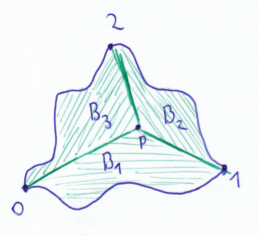
\includegraphics[scale=0.7]{doc-pics/pic-barycentric-curvilinear-definition.png}
    \caption{Definition of Barycentric Curvilinear Coordinates}
    %\label{fig:awesome_image}
\end{figure}

	\item For linear elements, the sum of barycentric coordinates always equals the total volume of the element for internal points, and is larger than that for external points. This is not true for non-convex elements, as the sum may be larger than the volume even for internal points. The method can not be improved by considering the sign of the barycentric coordinate based on the orientation of the boundary, as it is the same for internal and external points of the concave surface.
	\item Thus, if the sum of global barycentric coordinates is equal to the volume of the element, the point is automatically inside the element, otherwise we remain uncertain.
			
\end{enumerate}

\begin{figure}[!htb]
    \centering	
    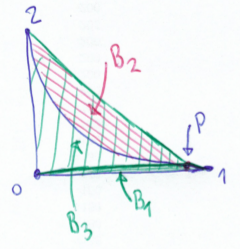
\includegraphics[scale=0.7]{doc-pics/pic-barycentric-problem-1.png}
    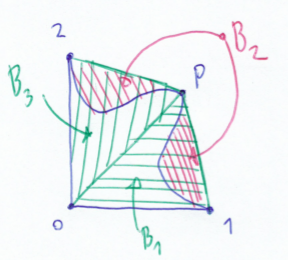
\includegraphics[scale=0.7]{doc-pics/pic-barycentric-problem-2.png}
    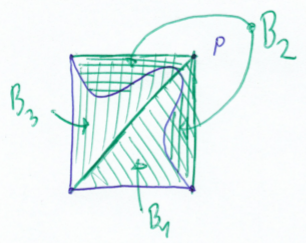
\includegraphics[scale=0.7]{doc-pics/pic-barycentric-problem-3.png}
    \caption{Problem cases with Barycentric Curvilinear coordinates}
    %\label{fig:awesome_image}
\end{figure}

\noindent
If both the above tests do not give a conclusive result, we need to use Global-To-Local mapping, and then $checkInside$ for the local coordinate. The challenges of this approach are described in the corresponding section. \\

\noindent
\textbf{Current Implementation: } There is no $is\_inside()$ method, only $local()$ method. Local method returns false if the point is not inside the element, and returns true and the correct local coordinate if it is. If the answer is true, we have to calculate the local coordinate anyway to make sure, makes sense to return it not to calculate it twice.

\begin{figure}[p]
    \centering
    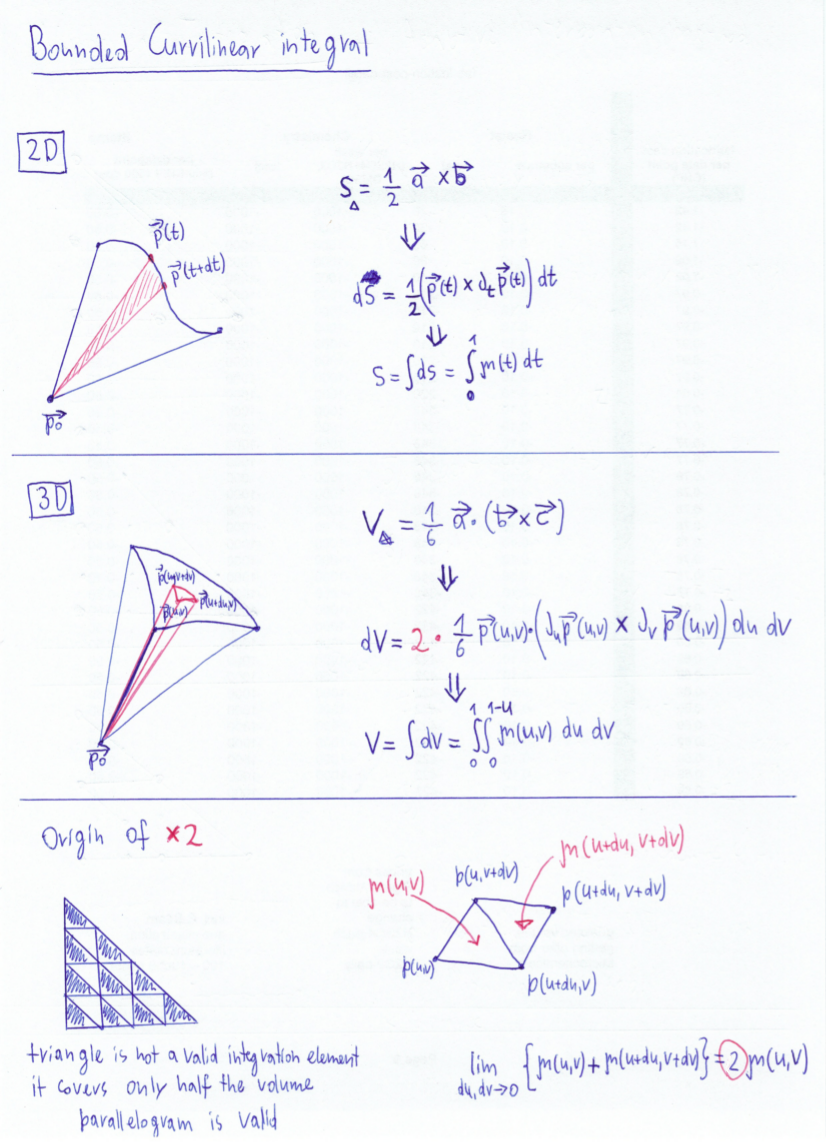
\includegraphics[scale=0.7]{doc-pics/pic-bounded-curvilinear-integral.png}
    \caption{Barycentric Coordinate Calculation}
    \label{fig:barycentric_coordinate_calculation}
\end{figure}


%%%%%%%%%%%%%%%%%%%%%%%%%%%%%%%%%%%%%%%%%%%%%%%%%%%%%%%%%%%%%%%%%%%%%
% Implementation Details - Curvilinear GMSH Reader
%%%%%%%%%%%%%%%%%%%%%%%%%%%%%%%%%%%%%%%%%%%%%%%%%%%%%%%%%%%%%%%%%%%%%

\section{Reading Curvilinear Grid}

% \subsection{Structure of .msh files}
% 
% \begin{mybox}
% \begin{lstlisting}
% $MeshFormat
% ver f_type data_size    # This line is mostly irrelevant
% $EndMeshFormat
% $Nodes
% n_vertices
% 1 x y z
% 2 x y z
% .......
% n_vertices x y z
% $EndNodes
% $Elements
% n_elem
% 1 elem_type n_tags (process_tags) v_1 v_2 ... v_N
% 2 elem_type n_tags (process_tags) v_1 v_2 ... v_N
% .......
% n_elem elem_type n_tags (process_tags) v_1 v_2 ... v_N
% $EndElements
% \end{lstlisting}
% \end{mybox}
% 
% \noindent
% where
% \begin{itemize}
% 	\item $ver$             - version of the GMSH file
% 	\item $f\_type$          - type of file (irrelevant)
% 	\item $data\_size$       - size of file (irrelevant)
% 	\item $n\_vertices$      - number of vertices of the mesh
% 	\item $i\ x\ y\ z$         - index of the vertex and its coordinates
% 	\item $n\_elem$          - number of elements of the mesh
% 	\item $elem\_type$       - Integer which determines element type and interpolation order
% 	\item $n\_tags$          - Total number of tags. If $>2$, then have $process\_tags$
% 	\item $process\_tags$    - Tags which determine the process the vertex belongs to. Only if GMSH is told to partition the mesh
% 	\item $v\_1\ v\_2\ ...\ v\_N$ - Indices of interpolatory vertices associated with this element (includes corners)
% \end{itemize}
% \subsection{Parallel Implementation}

From the outset the parallel implementation of the Curvilinear GMSH Reader is targeted at high parallel scalability. It loads the mesh evenly on all involved processes, avoiding master process bottlenecks. The algorithm to achieve this requires reading the mesh file several times on each process:

\begin{mybox}
\begin{enumerate}
  \item VERTEX PASS 1: Skip all vertices, and place file pointer before the element section

  \item ELEMENT PASS 1: Count the total number of elements and boundary segments

  \item ELEMENT PASS 2: Read corners for all elements within the block associated to this process. Given equal splitting of elements across all processes, the process with index $rank$ should read the elements with indices \[interv(rank) = \floor[\Big]{ [rank, rank+1] \cdot N_{elem} / p_{tot} } + 1.\]
        
  \item If partitioning is enabled, partition the elements among all processes. The partitioning uses the \textit{ParMETIS\_V3\_PartMeshKway} function of \ParMETIS{} \citeParMetis{}. It produces contiguous subdomains on each process, with a roughly equal number of elements on each process. \ParMETIS{} naturally also minimizes the number of boundary connections, thus minimizing the number of interprocessor boundaries and the amount of parallel communication necessary at a later stage. We have also implemented support for \ParMETIS{} multiple constraint partitioning capabilities, but, as of time of writing \ParMETIS{} does not guarantee contiguous subdomains for multi-constraint partitioning.
        
  \item ELEMENT PASS 3: Read all data associated with elements on this process partition. Map all faces to the elements sharing them using the sorted global index of the face corners. The elements are written to the grid factory
       
  \item ELEMENT PASS 4: Read all data associated with boundary elements. Determine if the element belongs to this process by looking it up in the available face map. Separate the processed boundaries by boundary tag. Identify which of the boundary tags is associated with the domain boundary by determining the faces that have only one neighboring element across all processes, and sharing this information with all other processes. Thus each process is aware of all volume and boundary tags, even if there are no entities with this tag on the process. The boundary segments are written to the grid factory.

  \item VERTEX PASS 1: Read the coordinates of the vertices associated with the entities present on this process. The vertex coordinates are written to the grid factory.
\end{enumerate}
\end{mybox}

\noindent
The implementation has an option to directly output the processed mesh into $.VTK$ file set for debugging purposes.

% \begin{mybox}
% \noindent
% Currently using brute-force, because it is not much slower than improved for \\
% 
% \noindent
% \uline{Trivial Algorithm: (Complexity $O(12 N_{elem} N_{\beta} / p_{tot}^2)$)}\\
% \textit{Loop over all stored boundary elements $\beta_i$, and over all stored internal elements $E_j$.} \\
% \textit{ If $\beta_i \in E_j$ for some $j$ then store $\beta_i$ }\\
% 
% \noindent
% \uline{Improved Algorithm: (Complexity $O(12 N_{elem} \log_2 (N_{\beta} / p_{tot}) / p_{tot}$)}\\
% 
% \begin{enumerate}
% 	\item Construct map from boundary vertex index set to boundary id
% 	\item Add all boundaries to the map
% 	\item Loop over each face of all internal elements
% 	\begin{enumerate}
% 		\item If $map[face]$ is non-null, link the element and boundary
% 	\end{enumerate}
% \end{enumerate}
% 
% \end{mybox}	
% 		
% \begin{enumerate}[resume]
% 	\item Add internal elements to factory
% \end{enumerate}
% \begin{mybox}
% 	\begin{itemize}
% 		\item For debugging purposes write each element to a .vtk file using CurvilinearVTKWriter.
% 		\item Add element vertices and global element index to factory
% 		\item If creating grid with boundaries, also pass $internal\_to\_boundary\_element\_linker$. This array stores the indices of boundaries which are connected to this element (if any).
% 	\end{itemize}
% \end{mybox}



%%%%%%%%%%%%%%%%%%%%%%%%%%%%%%%%%%%%%%%%%%%%%%%%%%%%%%%%%%%%%%%%%%%%%
% Implementation Details - Curvilinear Grid Constructor
%%%%%%%%%%%%%%%%%%%%%%%%%%%%%%%%%%%%%%%%%%%%%%%%%%%%%%%%%%%%%%%%%%%%%

\section{Constructing Curvilinear Grid}

The grid construction is called by the \textit{Grid Factory} (see \ref{interface-grid-factory}) after all the vertices, elements and boundary segments have been inserted. The construction of the \curvgrid{} is in accordance with the following plan

\begin{mybox}
\begin{enumerate}
	\item Construction of grid entities - Interior ($I$), Process Boundary ($PB$), Domain Boundary ($DB$) and Interior Boundary ($IB$) edges and faces.
	\item Construction of the global index for all entities. By default, the global index for vertices and elements is re-used from the mesh file.
	\item Construction of Ghost elements ($G$)
	\item Construction of entity subsets used for iteration over different entity partition types and codimensions
	\item Construction of communication maps, used to perform communication via the \textit{DataHandle} interface
	%\item Construction of OCTree for hierarchical element location
\end{enumerate}
\end{mybox}


\subsection{Storage}
\label{impl-grid-storage}

\noindent
The paradigm used in \curvgrid{} is to store all data corresponding to the grid in a single class, namely the \textit{CurvilinearGridStorage} class. Entities of each codimension are stored in arrays indexed by the local entity index, which is contiguous and starts from 0 on all processes. Each entity stores its global index, geometry type and partition type. For the detailed explanation on the correct assignment of partition types to entities of each codimension, the user is referred to the corresponding section of \dune{} grid usage manual, found on the website of the project. Elements and faces also store the associated material (physical) tag. Elements store the local index of all interpolatory vertices in the \textit{Sorted Cartesian} order (see \cref{impl-gmsh-numbering-convention}). The edges and faces do not store the interpolatory vertex indices, as it would be wasteful for higher curvilinear orders. Instead, each edge and face is stored as a subentity of an associated parent element - any of the elements containing it. Thus, each subentity stores the parent element local index, as well as the subentity index, by which the subentity is indexed within the reference element. Finally, each face stores its boundary type - Interior, Domain Boundary or Periodic Boundary, as well as the index of the 2nd parent element that shares it. By convention, the primary parent element must always be interior to the process storing the face. The secondary parent element may be either interior, or Ghost (\cref{fig:impl:ghostelements}). The data associated with a Ghost element is stored on the neighboring process, but can be accessed from this process as part of interprocessor communication. In case of Domain Boundaries, there is no secondary parent. By convention, any attempts to access the secondary parent of a Domain Boundary result in an exception, as the user code must take the provided partition type into account when addressing neighboring entities. \\

\noindent
\curvgrid{} contains several different local index sets, designed to uniquely index only the entities of a given subset. Namely, Domain Boundary segments, Interior Boundary segments, Process Boundaries, remaining Interior boundaries, as well as Ghost elements each have their own local index. \curvgrid{} provides maps between those indices and local indices of all entities of a given codimension. In addition, there is a unique index for grid corners, namely the interpolatory vertices that define the linear entities (\cref{fig:impl:storage:vertexvscorner}). This is necessary, because the \dune{} facade class operates in terms of linear elements, and thus requires a contiguous index for the corners. Importantly, among all vertices only entity corners possess unique process boundary index, since, for all interprocessor communication purposes, the mesh can be assumed to be linear without loss of generality. Finally, a map from global to local index is provided for entities of all codimensions. \\

\begin{figure}
    \centering
	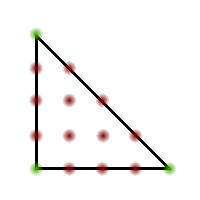
\includegraphics[scale=1.5]{images/vertex-vs-corner}
	\caption{The interpolatory vertices of the 5th order curvilinear triangle. Corners are given in red}
	\label{fig:impl:storage:vertexvscorner}
\end{figure}

\noindent
\curvgrid{} operates with two different types of \textit{GlobalIds}, designed to uniquely identify the entity among all processes. First of all, it is a pre-requisite that all vertices have an associated global index, which is either re-used from the mesh file, or constructed in the beginning of the grid construction procedure. Before the global indices for other codimensions are generated, these entities are uniquely identified by the sorted set of global indices of the entity corners, which can be used in a map to determine if a given communicated entity is already present on the receiving process. Later, when entities of all codimensions possess global index, the \textit{GlobalId} is simply a wrapper of the global index, such as to use minimal amount of resources necessary. It is the latter \textit{GlobalId} that is made available for the user code at the end of construction procedure. \\

\noindent
For the purposes of iterating over frequently used entity subsets, the corresponding local index subsets are provided for each codimension. Namely, subsets are provided for all entities of a given codimension, Interior entities, Process Boundary entities, Domain Boundary entities, Ghost entities, Interior + Domain Boundaries (called \textit{interior} in \dune{}), Interior + Domain Boundaries + Process Boundaries (called \textit{interior border} in \dune{}). \\

\noindent
For communication purposes, all communicating entities need to store a vector of ranks of processes with which these entities are shared. For more details on communicating entities, see \cref{impl-grid-constructor-comm}.




\subsection{Global index construction}
\label{impl-grid-constructor-globalindex}

\noindent
In this section we briefly describe the algorithm used to construct the global indices for all codimensions. The challenge in computing the global indices comes from the fact that originally the processes are not aware of their neighbors. Due to the insertion of complete boundary segments by the grid factory, each process can readily identify all of its process boundaries as the faces that have only one containing element on the process and are not already marked as domain boundaries. The algorithm has four definite stages - determining the neighboring process for each process boundary, assigning (virtual) ownership of each shared entity to only one of the processes sharing it, enumerating the global index on processes owning the entities, and communicating the global index to all other processes containing each shared entity. \\

\noindent
The algorithm starts by determining neighbor ranks of each Process Boundary ($PB$) corner. Currently, each process communicates all process boundary corner global indices to all other processes. From the received global indices each process can deduce all other processes sharing each of its corners. Then, each process assigns provisional neighbor processes to edges and faces by considering the processes that share all entity corners. If two processes share all the corners of a given entity, it does not mean that they share the entity as well (\cref{fig:impl:globalindex:fakeedge}). The ambiguity is quite rare, because most entities are shared only by two processes, and since each process boundary entity must be shared by at least two processes, there is no need to check if the entity exists. Nevertheless, the grid must be able to handle the rare case of an entity being shared by more than two processes. In this case, the edge and face \textit{GlobalIds} (see \cref{impl-grid-storage}) are communicated to all provisional neighboring processes. Each of the provisional neighbor processes then responds, whether or not each entity corner set corresponds to an entity. The ranks that are not confirmed to share the entities are then removed from the neighbor list. \\

\begin{figure}
    \centering
	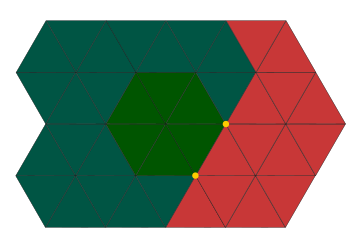
\includegraphics[scale=0.5]{images/parallel-fake-edge}
	\captionsetup{width = 0.8\textwidth}
	\caption{The two yellow vertices are shared between three processes. The edge in-between them only exists on red and green processes, but not on the blue one}
	\label{fig:impl:globalindex:fakeedge}
\end{figure}

\noindent
For each $PB$ edge and face, an owner is determined. The ownership strategy is flexible, as long as all processes agree. Currently, a shared entity is considered to be owned the process with the lowest rank among those sharing it. Each process owns all of its non-shared entities. The number of entities owned by each process is then communicated to all other processes. \\

\noindent
Each process then locally enumerates the global index of all its entities. To begin with, each process computes the shift in global index due to the entities of each codimension enumerated by the processes with ranks lower than this process rank. All processes enumerate global indices consecutively, starting with 0 on rank 0 process. This constructs a global index individually for each codimension. A global index over all entities is also constructed, shifting the enumeration also by all the enumerated entities of higher codimension. \\

\noindent
The enumerated global indices are then communicated among all processes sharing the entities. By analyzing entity neighbors, each process can compute how many global indices it needs to send to and receive from each other process, avoiding extra communication. At the end of this process, the global-to-local index map is filled on each process.


\subsection{Periodic boundary construction}
\label{impl-grid-constructor-periodic}

A recent feature of the \curvgrid is the Periodic Boundary Condition (PBC) support for cuboid domains. It is possible to have any 1, 2 or 3 dimensions periodic. \curvgrid supports Periodic Boundaries and the associated Ghost Entities. \\

\noindent
In order to generate a Periodic mesh it is sufficient to provide a periodic-conformal .msh file. This means that the Domain Boundary must be a cuboid surface, and all faces on parallel cuboid planes, for which periodicity is specified, should be conformal. That is, the conformal faces must exactly match via translation along the orthogonal axis (\cref{fig:impl:periodicconformal}). There is no need to provide any periodicity information in the .msh file - the periodic faces are recognized automatically. In order to inform the grid constructor of the periodicity, it is sufficient to pass to the \textit{CurvilinearGridFactory} an additional parameter, denoting which dimensions are expected to be parallel (see \cref{interface-grid-factory}) \\

\begin{figure}
    \centering
	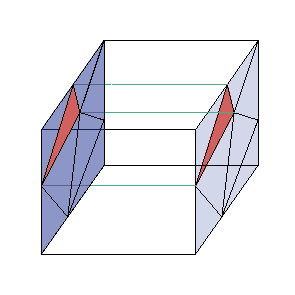
\includegraphics[scale=1.5]{images/periodic-conform}
	\captionsetup{width = 0.8\textwidth}
	\caption{The image demonstrates that a conformal periodic face pair is such that one of them can be obtained from the other through translation along the periodicity axis}
	\label{fig:impl:periodicconformal}
\end{figure}


\noindent
Currently the construction of the periodic boundary relies on gathering all the periodic faces on the master process, determining periodic neighbors, and scattering the neighboring information to the boundary owner processes.

\begin{mybox}
\begin{enumerate}
 \item Master process gathers the global indices of all periodic boundary faces, as well as their corner coordinates. 
 \item It separates all periodic faces into 6 arrays, with normals $-X$, $+X$, $-Y$, $+Y$, $-Z$, $+Z$ (non-periodic dimensions are ignored)
 \item For each periodic face the Center of Mass (CoM) is calculated, and each array is sorted w.r.t center of mass.
 \item If the mesh is indeed conformal, the each two arrays of opposite normals should now have the periodic neighbors in exactly the same order. Thus the periodic face pairs are found.
 \item For each face pair, the corresponding vertices are matched by checking that the vector connecting them is collinear with the face normal. The relative permutation index of vertices is calculated
 \item For each process its periodic neighbor information is communicated - the neighbor global index pair, as well as the permutation index.
\end{enumerate}
\end{mybox}

\noindent
IMPORTANT NOTE: The orientation of each boundary face is determined by the reference subentity orientation of the corresponding element, and thus does not follow any global pattern. Thus, any two periodic neighbor faces are conformal up to a permutation of indices. Since the grid element vertex indexing does not change, the permutation of indices also stays the same. It is therefore essential for each process to know the permutation that needs to be applied to its periodic face, such that it matches to the periodic face of the neighbor process. It is later used in the intersection implementation to link together the local indices of the neighboring elements within the shared face. \\

\noindent
It is important to note that the intersection is viewed as a subentity of its inner neighbor element. Should we construct the intersection of the other neighboring element (for which it will be the inner element), corresponding to the same face, the orientation of the face may change, depending on the vertex ordering of that element. The typical way to perform the face orientation matching for neighbor elements in \dune{} is to construct neighboring local geometries \textit{geometryInInside} and \textit{geometryInOutside} for each intersection. These geometries are maps from the local coordinate of a face to the corresponding local coordinate of the containing element, namely

\begin{mybox}
\begin{lstlisting}
  LocalCoordinate3D insideElementLocalCoordinate = geometryInInside. global(localFaceCoordinate)
\end{lstlisting}
\end{mybox}

\noindent
The above design pattern makes use of two important observations
\begin{itemize}
 \item The coordinates of the \textit{geometryInInside} are a subset of the coordinates of a 3D reference element, which exactly correspond to the corners of the face, viewed as a subentity of the inner reference element.
 \item The coordinates of the \textit{geometryInOutside} are a subset of the coordinates of a 3D reference element, which exactly correspond to the corners of the face, viewed as a subentity of the outer reference element, followed by a permutation. The permutation the permutation that needs to be applied to the corners of the face, as seen from the inner element, to correspond to the corners of that face, as seen from the outer element.
\end{itemize}

\noindent
For example, a given face is the $s0=$2nd subentity of the inner element, and the $s1=$0th subentity of the outer element (out of 4 possible). Also, assume that the order of vertices in inner and outer elements is such, that the corners of the face as seen from the inner element would map to the corners, as seen from the outer element as $M = (0,1,2) \rightarrow (2,0,1)$. As of time of writing, the \dune{} tetrahedral reference element is such, that its corner coordinates are $pref=\{(0.0\ 0.0\ 0.0), (1.0\ 0.0\ 0.0), (0.0\ 1.0\ 0.0), (0.0\ 0.0\ 1.0)\}$ and the indices corresponding to the reference subentity faces are $fref=\{(0 1 2), (0 1 3), (0 2 3), (1 2 3)\}$. Thus, the corners of the \textit{geometryInInside} are

\begin{mybox}
\begin{lstlisting}
 pref[fref[s0]] = pref[fref[2]] = {pref[0], pref[2], pref[3]}
   = {(0.0 0.0 0.0), (0.0 1.0 0.0), (0.0 0.0 1.0)}
\end{lstlisting}
\end{mybox}

\noindent
and of the \textit{geometryInOutside} are
\begin{mybox}
\begin{lstlisting}
 M[pref[fref[s1]]] = M[pref[fref[0]]]
   = M[{pref[0], pref[1], pref[2]}] = {pref[2], pref[0], pref[1]}
   = {(0.0 1.0 0.0), (0.0 0.0 0.0), (1.0 0.0 0.0)}
\end{lstlisting}
\end{mybox}

\noindent
Currently in \curvgrid{}, for the entities that share a face, the necessary permutation is generated upon construction of the intersection, by simply matching the local indices of the face, as seen from inner and outer neighbor elements. For the periodic boundaries, this information might not be locally available, if ghost elements are not constructed, and the determination of the permutation is a tedious procedure with multiple floating point comparisons. Thus, for periodic boundaries, the permutation index is calculated once during the construction, then stored and reused for intersection construction. \\

\noindent
As a result, calculating coupling integrals over any intersection, including periodic, follows exactly the same procedure, and no additional effort is necessary from the user (see tutorial \cref{usage-howto-tutorial-periodic}) \\



\subsection{Ghost element construction}
\label{impl-grid-constructor-ghost}

\noindent
Ghost entities are the subentities of the element on the other side of the process or periodic boundary face, including the element itself. The process and periodic boundary entities themselves can be part of a Ghost entity, but are not considered Ghost entities. Thus, the Ghost entities are the entities of \textit{InteriorBorder} partition (on their parent process) normally not present on this process, but are borrowed by this process. On the borrowing process, the ghost entities have the partition type \textit{GhostEntity}. The ghost entities due to a periodic boundary are treated exactly the same way as those due to a process boundary, with the exception that all of the process boundaries of a ghost element are the same local process boundaries, whereas for each periodic boundary a ghost element has another ghost face, which corresponds to that periodic boundary, but is disjoint from it, and has different local and global index (\cref{fig:impl:periodicvsprocessboundary}). Another special case are the ghost elements of the periodic boundaries, for which the periodic neighbor element is also local to the same process. In this case, no \textbf{ghost element is constructed}, and no entities are copied. The outer neighbor element of the periodic boundary in that case is simply specified as the local element on the other side. Local periodic neighbors are treated during the periodic construction \cref{impl-grid-constructor-periodic}, whereas this section only deals with non-local periodic neighbors. \\

\noindent
Construction of Ghost entities involves communicating all the information associated with the entities to the neighboring processes, and then incorporating the Ghost entities into the grid on the receiving side (\cref{fig:impl:ghostelements}). \\

\begin{figure}
    \centering
	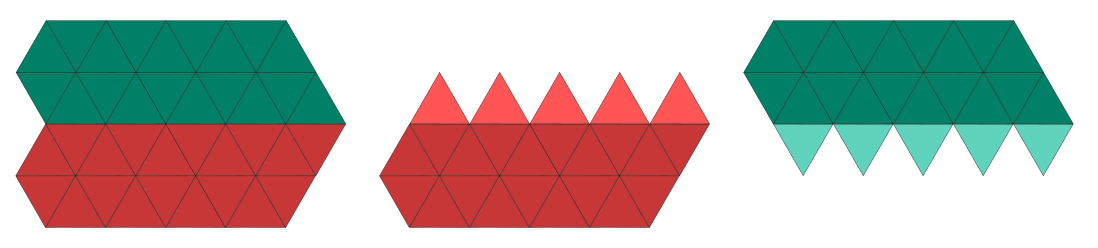
\includegraphics[scale=0.5]{images/parallel-ghost-elements}
	\caption{The first image depicts two neighboring processes without Ghost elements. The second and third images contain only the first and only the second process entities respectively, including Ghost elements borrowed from the other process. }
	\label{fig:impl:ghostelements}
\end{figure}

\begin{figure}
    \centering
	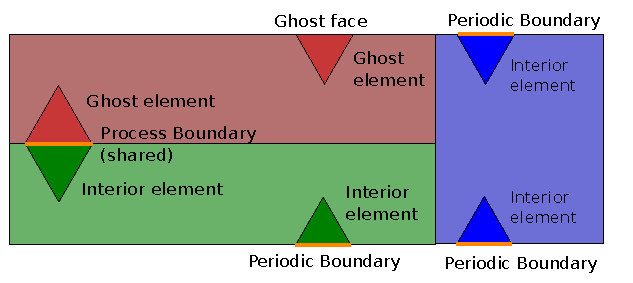
\includegraphics[scale=1.5]{images/periodic-vs-process-boundary}
	\captionsetup{width = 0.8\textwidth}
	\caption{This image explains the difference between process boundary ghost elements (left), periodic ghost elements (center), and local periodic neighbors(right). In the left-most image, the green process borrows an element from the red process via a process boundary. That element becomes a ghost. Both the interior green element and the ghost element share the yellow process boundary face. In the center, the green process borrows an element from the red process via a periodic boundary. That element becomes a ghost. The ghost element stays in the same geometric position, and is completely disjoint from its periodic neighbour. The right-most image demonstrates periodic neighbour elements for the case, when both neighboring periodic boundaries are on the same process (blue). In this case, nothing is borrowed or copied, only that each of the neighboring elements considers the other a neighbor. It is important to note that both the coordinates and the global and local indices of periodic neighbors are completely disjoint, thus allowing to address these entities individually. }
	\label{fig:impl:periodicvsprocessboundary}
\end{figure}

\noindent
Since for every $PB$ and \textit{Periodic} face the neighboring process rank has already been determined in the previous sections, and the global index is already known, it remains only to communicate the corresponding neighbor entities and correctly integrate them into the local grid. Firstly, one needs to communicate the properties of the structure to be communicated. Thus, for each interior element next to the boundary the interpolation order is communicated, as well as the number of boundary faces it shares with the receiving side. It is important to note that a Ghost element can have more than one boundary face associated to it, and the receiving side does not know in advance if one, two or three of its boundary faces are associated with the same Ghost element on the other side. This is also the reason it is not possible to know in advance how many ghosts will be received from a neighbor process. Afterwards, for each Ghost element the global index, physical tag, global indices of all codimension subentities and subentity indices of boundary faces of the boundary-interior elements are communicated. The corresponding Ghost elements are then added to the mesh, and it is determined which vertex coordinates are missing. The vertex coordinates are not communicated immediately, because the neighbor process may already have some of the global coordinates due to narrow mesh appendices. Thus, each process communicates the number of vertex coordinates missing from each of its neighbors, and then communicates the missing coordinates.




\subsection{Communication interface construction}
\label{impl-grid-constructor-comm}

The communication paradigm of \dune{} \textit{DataHandle} interface is to communicate data between instances of the same entity on different processes. Depending on the communication protocol, only entities of specific structural types will communicate. We will slightly redefine the partition type classes in this section for compactness reasons. There are three different communicating partition types
\begin{itemize}
	\item $PB$ - Process boundary entities, that is, process boundary faces and their subentities
	\item $I$ - Interior entities, including the $DB$ but excluding the $PB$ entities.
	\item $G$ - Ghost elements and their subentities, excluding $PB$
	\item $PERB$ - Periodic Boundaries
\end{itemize}


\begin{figure}
    \centering
	\begin{subfigure}[b]{0.48\textwidth}
	  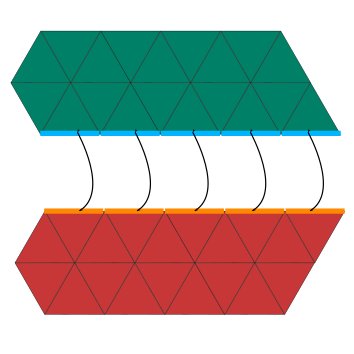
\includegraphics[scale=0.4]{images/parallel-comm-PBPB}
	  \captionsetup{width=0.8\textwidth} 
	  \caption{$PB \leftrightarrow PB$. Communication of neighboring process boundaries}
	\end{subfigure}
	\begin{subfigure}[b]{0.48\textwidth}
	  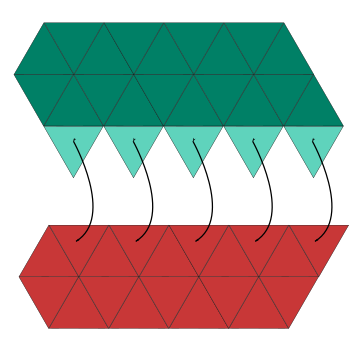
\includegraphics[scale=0.4]{images/parallel-comm-IG}
	  \captionsetup{width=0.8\textwidth} 
	  \caption{$I \leftrightarrow G$. Communication of interior element and its Ghost on another process }
	\end{subfigure}
	\begin{subfigure}[b]{0.48\textwidth}
	  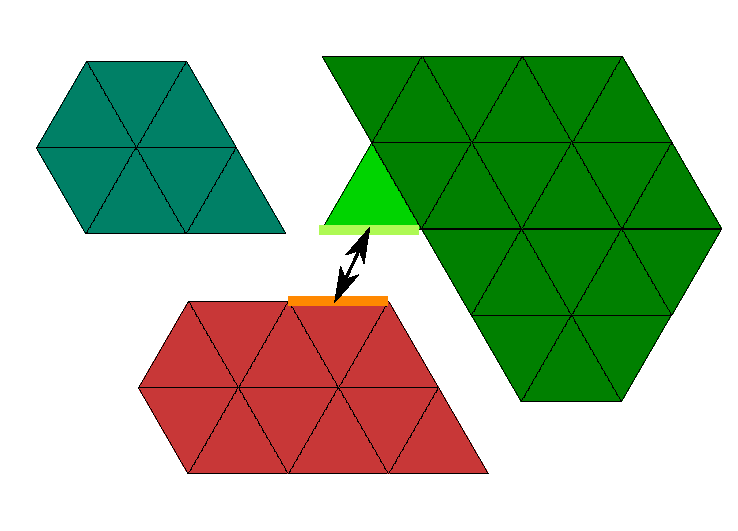
\includegraphics[scale=0.4]{images/parallel-comm-PBG}
	  \captionsetup{width=0.8\textwidth} 
	  \caption{$PB \leftrightarrow G$. Communication of a Ghost of the blue process on the green process with a process boundary on the red process}
	\end{subfigure}
	\begin{subfigure}[b]{0.48\textwidth}
	  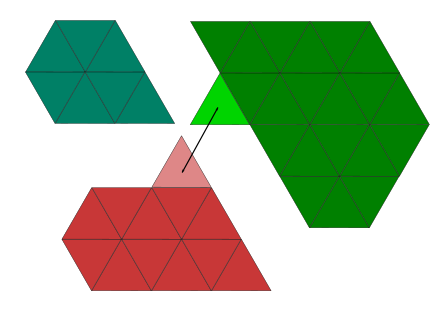
\includegraphics[scale=0.4]{images/parallel-comm-GG}
	  \captionsetup{width=0.8\textwidth} 
	  \caption{$G \leftrightarrow G$. Communication between two ghosts of the same element of the blue process on the green and the red process}
	\end{subfigure}
	\captionsetup{width=0.8\textwidth}
	\caption{ Partition type pairs that can communicate to each other}
	\label{fig:impl:comm:partitionpairs}
\end{figure}

\noindent
A special case is the recently added periodic communication $PERB \rightarrow PERB$. Currently it is only implemented for periodic faces (not yet the edges and vertices). Each periodic boundary communicates with its neighbor on the other process. By convention, if both periodic boundaries are on the same process, they do not communicate, as that would result in entities sending data to themselves. Also, the user must be aware that in all cases except the periodic communication the sending and receiving entities have the same global index, and the same position in space. The periodic boundaries communicate to each other, while being spatially-separated, and having different global indices. Note also, that ghost elements generated by periodic boundaries also participate in all above protocols, and are in principle the same, as the ghosts, generated by the process boundaries, except that they are disjoint from the boundary (see \cref{fig:impl:periodicvsprocessboundary}). \\


\noindent
We consider all partition type pairs, for which the \textit{DataHandle} communication is possible (\cref{fig:impl:comm:partitionpairs}). Note that interior entities only communicate to Ghost and vice-versa, because Process Boundaries are Process Boundaries on both neighboring processes. However, Process Boundaries can communicate to Ghosts and vice-versa, because a process boundary can be a Ghost with respect to a third process at the triple point. \\

\noindent
The \textit{DataHandle} interface foresees four communication protocols. The \cref{table:impl:datahandle:protocols} presents the communication interfaces used by Dune, and explains how they translate to communication between entities of above specified partition types \\

\begin{table}
\centering
\begin{tabular}{ | l | l | l | l | l | l | l | l | }
  \hline
  Interface & Direction &
      \small $PB \rightarrow PB$ \normalsize &
      \small $PB \rightarrow G$ \normalsize &
      \small $I \rightarrow G$ \normalsize &
      \small $G \rightarrow I$ \normalsize &
      \small $G \rightarrow PB$ \normalsize &
      \small $G \rightarrow G$ \normalsize \\ \hline 
  \begin{tabular}[x]{@{}c@{}}\lstinline|InteriorBorder_|\\ \lstinline|InteriorBorder| \end{tabular}
  & ---      & Y & N & N & N & N & N \\ \hline
  \lstinline|InteriorBorder_All|            & Forward  & Y & Y & Y & N & N & N \\ \hline
  \lstinline|InteriorBorder_All|            & Backward & Y & N & N & Y & Y & N \\ \hline
  \lstinline|All_All|                       & ---      & Y & Y & Y & Y & Y & Y \\ \hline
\end{tabular}
\caption{Communication interfaces of \textit{DataHandle}, and the associated communicating partition type pairs}
\label{table:impl:datahandle:protocols}
\end{table}


\noindent
The aim of this part of the grid constructor is to generate/reuse unique index maps for the sets $PB$, $I$ and $G$. Then, for every communicating entity, for every possible partition type pair, we require an array of ranks of the processes for which such communication is possible. Note that the map for the pair $PB\rightarrow PB$ already exists, it is constructed in the very beginning of the grid construction procedure to enable global indices and Ghost elements. The algorithm is as follows:

\begin{mybox}
\begin{enumerate}
	\item Mark the neighbor process ranks of the associated $PB$ for all $I$ and $G$ entities, whose containing elements neighbor $PB$, thus enabling the $I \rightarrow G$ and $G \rightarrow I$ communication. Note that entities of all (!!) codimensions can have more than one neighbor rank obtained this way. During the marking, elements with two or more process boundaries from different processes may be encountered. In that case, for each process boundary entity the rank of the other process boundary is marked, thus providing some information for the future construction of the $PB \rightarrow G$ communications.
	\item Then, all entities that can communicate are associated with ranks of all other processes, over which the entities are shared.% It remains to finish the $PB \rightarrow G$ communication, and calculate the remaining protocols $G \rightarrow I$, $G \rightarrow PB$ and $G \rightarrow G$.
	\item For all $PB$ entities, subtract $PB\rightarrow PB$ set from the $PB \rightarrow G$ set to ensure that the latter excludes the former. Also, mark the number of effective $PB \rightarrow G$ candidate entities of each codimension for each process
	\item For all $PB$ entities with non-empty $PB \rightarrow G$ set, communicate $G$ indices to all neighboring $PB$ entities
	\item For all $PB$, append the union of the received $G$ to the $PB \rightarrow G$ set, thus completing it %(hopefully)
	\item For all $PB$ entities with non-zero $PB \rightarrow G$, communicate self index to all $G$ of $PB \rightarrow G$ set
	\item For all $G$, append the union of the received $PB$ to the $G \rightarrow PB$ set, thus completing it %(hopefully)
	\item For all $PB$ entities with non-zero $PB \rightarrow G$, communicate to all own $G$ neighbors all the other $G$ in the set
		%\subitem Optimization - do this only if you are lowest rank among all $PB$-neighbors
		%\subitem Further optimization - do this only if you are modulus-rank among all $PB$-neighbors
	\item For all $G$, append the union of the received $G$ to the $G \rightarrow G$ set, thus completing it %(hopefully)	
\end{enumerate}
\end{mybox}



    


% 
% \subsection{Iteration set construction}
% \label{impl-grid-constructor-iterator}
% 
% Construction of the iterator sets involves simply iterating over all entities, and filling the sets with local indices based on the entity structural type.
% 
% 
% \subsection{OCTree construction}
% \label{impl-grid-constructor-octree}








%%%%%%%%%%%%%%%%%%%%%%%%%%%%%%%%%%%%%%%%%%%%%%%%%%%%%%%%%%%%%%%%%%%%%
% Implementation Details - Curvilinear VTK Writer
%%%%%%%%%%%%%%%%%%%%%%%%%%%%%%%%%%%%%%%%%%%%%%%%%%%%%%%%%%%%%%%%%%%%%

\section{Writing Curvilinear Grid}

For the grid output, two hierarchic classes have been implemented - \textit{CurvilinearVTKWriter} and \textit{CurvilinearVTKGridWriter}. The former discretizes and accumulates entities and fields one-by-one and later writes them, and the latter uses the former to write the entities of the grid by iterating over them. The implementation of the \textit{CurvilinearVTKWriter} is best understood by considering its features.


\begin{enumerate}  
  \item \textit{nodeSet} is a vector of global coordinates of interpolatory vertices of the entity in correct order \ref{impl-gmsh-numbering-convention}
  \item \textit{tagSet} is a set of 3 scalar fields used for diagnostics, which typically accompany all written elements. Namely, they are the physical tag, the partition type, and the containing process rank in that very order. 
  \item \textit{interpolate} parameter determines how the virtual refinement of the entity is performed. If true, the regular grid of interpolatory points is re-used to subdivide the entity into smaller linear entities. If false, a new regular grid is constructed for this purpose, using the \textit{nDiscretizationPoint} parameter to determine the number of desired discretization vertices per edge. If the interpolation vertices are used the latter parameter is discarded. Note that the associated fields are sampled over the vertices of the virtual refinement grid, and thus increasing the virtual refinement is useful for better visualizing the element curvature and/or finer field resolution. Note that increasing \textit{nDiscretizationPoint} results in quadratic increase in both writing time and the resulting visualization file size, so the parameter must be used with care.
  \item \textit{explode} optional parameter shrinks all entities with respect to their mass-centers, allowing to better visualize the 3D structure of the grid. Default parameter is $0.0$, which corresponds to no shrinking, and the maximum allowed parameter is $0.99$
  \item \textit{magnify} optional parameter expands all boundary surfaces with respect to the origin, allowing to better visualize the difference between boundary segments and element faces. By default there is no magnification  
  \item \textit{writeCodim} is a vector of 4 boolean variables, one for each entity codimension. This vector allows the user to control the specific codimensions of entities to be displayed. For example, it is possible to switch on only the edge wireframe of the mesh by providing $\{ false, false, true, false \}$
\end{enumerate}


\begin{figure}
	\centering
	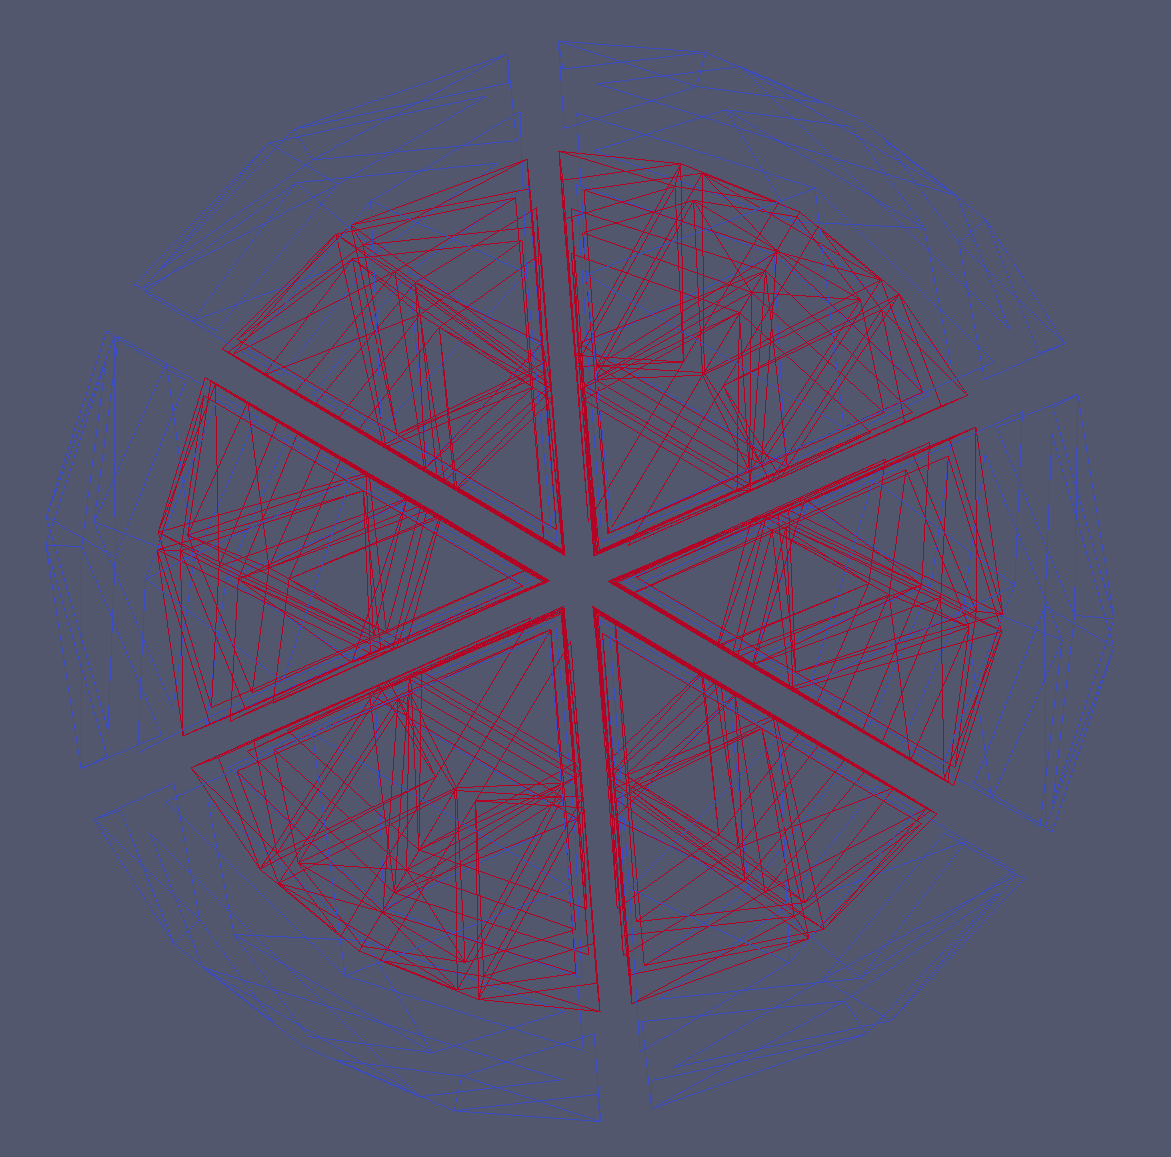
\includegraphics[scale=0.2]{images/gmshreader-vtk-wireframe}
	\caption{Visualization of an edge wireframe of a 32 element 2nd order mesh using the manual virtual refinement with  \textit{nDiscretizationPoint=3}  }
	\label{fig:gmshreader:wireframe}
\end{figure}


% \subsection{Optimal Sampling Rate}
% 
% Here we would like to discuss how many sampling points are required to represent the bounded curve using linear interpolation. This is necessary, for example, for visualisation. For a line segment, interpolating the curve bounded by 2 points, the analytic error is bounded by
% \begin{equation}
% 	\epsilon = |f(x) - g(x)| \leq \frac{1}{8} \max_{z \in [x_a, x_b]} \{ g''(z)  \} (x_a - x_b)^2
% \end{equation}
% \noindent
% where $f(x)$ is the line segment, $g(x)$ is the original function. $x_a$ and $x_b$ are arguments of the endpoints of the interval. \\
% 
% \noindent
% Given a large interval $L$ which we split into $N$ equal segments such that $x_b - x_a = L/N$, the maximal error over all interpolated intervals is bounded by
% \begin{equation}
% 	\epsilon_{\max} \leq \frac{L^2}{8 N^2} \max_{z \in L} \{ g''(z) \}
% \end{equation}
% \noindent
% This can be rewritten to obtain the necessary interval number per edge
% \begin{equation}
% 	N = \biggl \lceil \alpha \sqrt{ \max_{z \in L} \{ g''(z) \} } \biggr \rceil
% \end{equation}
% \noindent
% where $\alpha$ depends on precision and length of the interval. We observe that there is a problem with this formula, namely that if $g''(z) = 0$ we get 0 intervals, and if $g''(z)$ is small, we get 1 interval, and we would like 2, because there is at least some curvature, and it should be emphasized that the case is different from just straight line. Therefore we empirically modify the formula
% \begin{equation}
% 	N = \biggl \lceil \alpha \sqrt{ \max_{z \in L} \{ g''(z) \} } + 1 \biggr \rceil
% \end{equation}
% 
% \noindent
% Finally, since this equation is not exactly accurate for surfaces, and it is rather hard to make sense of optimal relative error, it is much easier to choose $\alpha$ empirically. We will generally operate with unit length edges ($L = 1$), and would like to, for example, have 5 points per edge with standard quadratic curvature $g(x) = x^2$. We obtain that $\alpha \approx 2.8$. \\
% 
% \noindent
% As a rule of thumb, we can calculate the expected number of intervals for a standard function $g(x) = \sum_i x^i$ using this formula. The first 5 orders will produce edge intervals $\{ 1, 5, 9, 17, 35\}$, which will correspond to the number of vertices per edge $\{ 2, 6, 10, 18, 36\}$, and thus the number of surface vertices ($i(i+1)/2$) will be given by $\{3, 21, 55, 171, 666\}$.



\section{Diagnostics tools}
\subsection{Mesh statistics}
\subsection{Visualisation}



\chapter{Tutorials}

%%%%%%%%%%%%%%%%%%%%%%%%%%%%%%%%%%%%%%%%%%%%%%%%%%%%%%%%%%%%%%%%%%%%%
% Curvilinear Grid Howto - Section on tutorials
%%%%%%%%%%%%%%%%%%%%%%%%%%%%%%%%%%%%%%%%%%%%%%%%%%%%%%%%%%%%%%%%%%%%%

\noindent
In order to start using the \curvgrid{} module we recommend to study the source code of the tutorials provided in \textit{curvilineargridhowto} folder. The tutorials use progressively more complicated concepts, so it is recommended to address them in the indexed order.


\subsection{Preliminaries - Creating Grid}
\label{usage-howto-tutorial-preliminaries}

All tutorials of \curvgrid{} reuse the simple auxiliary routine located in \textit{creategrid.hh}. This routine contains paths to all meshes currently used in tutorials, allowing the user to select the desired mesh by providing its index. It then proceeds to initialize the logging mechanisms
\begin{mybox}
\begin{lstlisting}
    Dune::LoggingMessage::init(mpihelper);
    Dune::LoggingTimer<Dune::LoggingMessage>::init(mpihelper);
\end{lstlisting}
\end{mybox}

\noindent
These singleton classes are essential for \curvgrid{}, as they support the parallel logging of the grid reading, construction and writing process, as well as later statistics on performance of individual routines. They can also be used by the user to write user logging output and time user functions, comparing them to the grid construction time. The next step is initializing the \textit{Curvilinear Grid Factory}

\begin{mybox}
\begin{lstlisting}
  Dune::CurvilinearGridFactory<GridType> factory(withGhostElements, withGmshElementIndex, mpihelper);
\end{lstlisting}
\end{mybox}

\noindent
where the boolean variable $withGhostElements$ determines whether the Ghost elements will be constructed and $withGmshElementIndex$ determines if the global element index from \gmsh{} is going to be reused by the grid (recommended). Otherwise, the index is automatically generated (see Tutorial 6 for discussion). After the above prerequisites, the curvilinear \gmsh{} reader is used to read the mesh file, partition it and write it to the provided grid factory.

\begin{mybox}
\begin{lstlisting}
  Dune::CurvilinearGmshReader< GridType >::read(factory, filename, mpihelper); 
\end{lstlisting}
\end{mybox}

\noindent
The \textit{Curvilinear Grid Factory} extends the interface of the standard dune grid factory, and therefore it will not work with other grids available in Dune. In order to achieve that, one must instead use the provided \textit{FactoryWrapper}. This wrapper class adheres to the standard grid factory interface, and disregards any process tag or curvilinear information provided by the curvilinear \gmsh{} reader. \\

\noindent
Finally, the grid is constructed, providing the user with the associated pointer. We note that the user must delete the grid pointer after use. %This is due to the fact that the factory used to create the grid ceases to exist before the grid itself.

\begin{mybox}
\begin{lstlisting}
  GridType *grid = factory.createGrid();
\end{lstlisting}
\end{mybox}

\subsection{Tutorial 1 - Getting started}
\label{usage-howto-tutorial-gettingstarted}

\noindent
This tutorial uses the above procedure to construct the \curvgrid{} by reading it from a \gmsh{} file. This and all other tutorials can be run both in serial and in parallel. First we define the grid

\begin{mybox}
\begin{lstlisting}
  typedef Dune::CurvilinearGrid<ctype, dim, isCached> GridType;
\end{lstlisting}
\end{mybox}

\noindent
where $dim=3$ is the dimension of the grid, $ctype=double$ is the underlying real type, and the $isCached$ is a boolean variable determining if the curvilinear geometry caching is used (recommended). Currently, only 3D tetrahedral grids are available. Then, the curvilinear grid is created by the $createGrid$ procedure described above. Finally, if we are interested in the time statistics for reading and construction of the grid, it can be obtained using the following command

\begin{mybox}
\begin{lstlisting}
  Dune::LoggingTimer<Dune::LoggingMessage>::reportParallel();
\end{lstlisting}
\end{mybox}



\subsection{Tutorial 2 - Traverse}
\label{usage-howto-tutorial-traverse}

This tutorial repeats the procedure from tutorial 1 to create the grid. It then iterates over the grid and extracts relevant information from the curvilinear entities. Currently, \curvgrid{} does not support refinement, so both leaf and level iterators will only iterate over the parent entities. As of \dune{} 2.4 revision the range-based for iterators introduced in \textit{c++11} standard are the preferred way to perform grid iteration. The below example iterator will iterate over all entities of the grid of a given codimension

\begin{mybox}
\begin{lstlisting}
  LeafGridView leafView = grid.leafGridView();
  for (auto&& elementThis : entities(leafView, Dune::Dim<dim - codim>())) {...}
\end{lstlisting}
\end{mybox}


Now, we would like to extract some relevant information from the iterator
\begin{mybox}
\begin{lstlisting}
  Dune::GeometryType gt = elementThis.type();
  LocalIndexType  localIndex
    = grid.leafIndexSet().index(elementThis);
  GlobalIndexType globalIndex
    = grid.template entityGlobalIndex<codim>(elementThis);
  PhysicalTagType physicalTag
    = grid.template entityPhysicalTag<codim>(elementThis);
  InterpolatoryOrderType interpOrder
    = grid.template entityInterpolationOrder<codim>(elementThis);
  BaseGeometry geom
    = grid.template entityBaseGeometry<codim>(elementThis);
  std::vector<GlobalCoordinate> interpVertices = geom.vertexSet()
\end{lstlisting}
\end{mybox}

\noindent
The $GeometryType$ and $LocalIndex$ are standard in \dune{}. $GlobalIndex$ provides a unique integer for each entity of a given codimension, over all processes. $PhysicalTag$ is the material tag associated with each entity, obtained from the mesh file. It can be used to relate to the material property of the entity, or to emphasize its belonging to a particular subdomain. In current \dunegrid{} standard this information can only be obtained by through the reader and requires auxiliary constructions. $InterpolatoryOrder$ denotes the integer polynomial interpolation order of the geometry of the entity. Currently, \curvgrid{} supports orders 1 to 5, the limiting factor being the curvilinear vertex indexing mapper in the reader. Finally, the $entityBaseGeometry$ gives the user direct access to the curvilinear geometry class of the entity, thus extending the interface provided by \textit{Dune::Grid::Geometry}. For example, it can be used to obtain the set of interpolatory vertices of the geometry, or an analytic polynomial matrix representing its Jacobian. \\






\subsection{Tutorial 3 - Visualization}
\label{usage-howto-tutorial-visualisation}

This tutorial demonstrates a simple way to output the curvilinear grid and associated vector fields (e.g. solutions of your PDE) to a PVTU file set using the \textit{CurvilinearVTKGridWriter} class. The writer is able to output arbitrary number of user-defined fields. The fields can be scalar or vector, and can be associated either with elements or with boundary faces. The sampled fields must overload the \textit{Dune::VTKScalarFunction} or \textit{Dune::VTKVectorFunction} standard provided by \curvgrid{}, and thus adhere to the following interface:

\begin{mybox}
\begin{lstlisting}
    // Writer initializes the functor once per each entity. This procedure can be used to pre-compute any quantities that do not change over the entity, accelerating the output
    virtual void init (const Entity & entity) {...}

    // Procedure that returns the field value as a function of local (!) coordinate
    virtual Range evaluate(const Domain & x) const  {...}

    // Procedure that returns the field name as it will appear in output file
    virtual std::string name() const  { return "localIndex2D"; }
\end{lstlisting}
\end{mybox}

\noindent
We provide 6 examples:
\begin{itemize}
  \item Element index scalar in 3D, written over all elements of the grid;
  \item Boundary segment index scalar in 2D, written over all boundary segments of the grid;
  \item Local sinusoidal vector in 3D, written over all elements of the grid;
  \item Local sinusoidal vector in 2D, written over all boundary segments of the grid;
  \item Global sinusoidal vector in 3D, written over all elements of the grid;
  \item Global sinusoidal vector in 2D, written over all boundary segments of the grid;
\end{itemize}

\noindent
These examples illustrate the important difference between local and global coordinates. Local coordinates are unique for each element, so one shall observe unique field behavior for each element. Global coordinates on the other hand are the same for all elements, thus providing a single continuous sinusoid across the entire mesh. The local fields are associated with the orientation of the element in space, which is arbitrary up to the permutation of element corners. Thus, to correctly display local fields, one must consider the orientation of the element. This can be achieved by considering the global coordinates and/or global indices of the corner vertices of the element, and of the intersection faces in between two elements. \\

\noindent
We start by constructing a curvilinear grid as previously demonstrated. We then proceed to initialize the writer, as well as fix its virtual refinement order to 15. We do this because we want to resolve the details of the sinusoid function to a very high precision, and because the mesh size is small. This operation is time-consuming, and, in general, the user should be aware of quadratic complexity of virtual refinement, and choose the refinement order that is necessary and sufficient. Should we choose to avoid specifying a fixed refinement order, the writer will calculate this order itself by considering the curvilinear order of the element. This works fine for most FEM applications, unless the basis order of the element is larger than its curvilinear order.

\begin{mybox}
\begin{lstlisting}    
  Dune::CurvilinearVTKGridWriter<GridType> writer(*grid);
    
  const int userDefinedVirtualRefinement = 15;
  writer.useFixedVirtualRefinement(userDefinedVirtualRefinement);
\end{lstlisting}
\end{mybox}

\noindent
We proceed to stack the pointers to the above field functors into 4 arrays, distinguished by vector/scalar and 2D/3D fields. We have decided to use dynamic polymorphism to implement this functionality. While this may be less efficient than other implementations, it allows writing fields produced by different functors by the very same compact routine.

\begin{mybox}
\begin{lstlisting}    
  std::vector<BaseVTKScalarFunction2D *> vtkFuncScalarSet2D_;
  std::vector<BaseVTKScalarFunction3D *> vtkFuncScalarSet3D_;
  std::vector<BaseVTKVectorFunction2D *> vtkFuncVectorSet2D_;
  std::vector<BaseVTKVectorFunction3D *> vtkFuncVectorSet3D_;

  vtkFuncScalarSet2D_.push_back(
    new VTKFunctionBoundarySegmentIndex<GridType>(*grid));
  vtkFuncScalarSet3D_.push_back(
    new VTKFunctionElementIndex<GridType>(*grid));

  vtkFuncVectorSet2D_.push_back(new VTKFunctionLocalSinusoidFace());
  vtkFuncVectorSet2D_.push_back(new VTKFunctionGlobalSinusoidFace());
  vtkFuncVectorSet3D_.push_back(new VTKFunctionLocalSinusoidElem());
  vtkFuncVectorSet3D_.push_back(new VTKFunctionGlobalSinusoidElem());

  writer.addFieldSet(vtkFuncScalarSet2D_);
  writer.addFieldSet(vtkFuncScalarSet3D_);
  writer.addFieldSet(vtkFuncVectorSet2D_);
  writer.addFieldSet(vtkFuncVectorSet3D_);
  writer.write("./", "tutorial-3-output"););
\end{lstlisting}
\end{mybox}
	
	
\begin{figure}[H]
	\begin{subfigure}[b]{0.45\textwidth} \hspace{4mm} 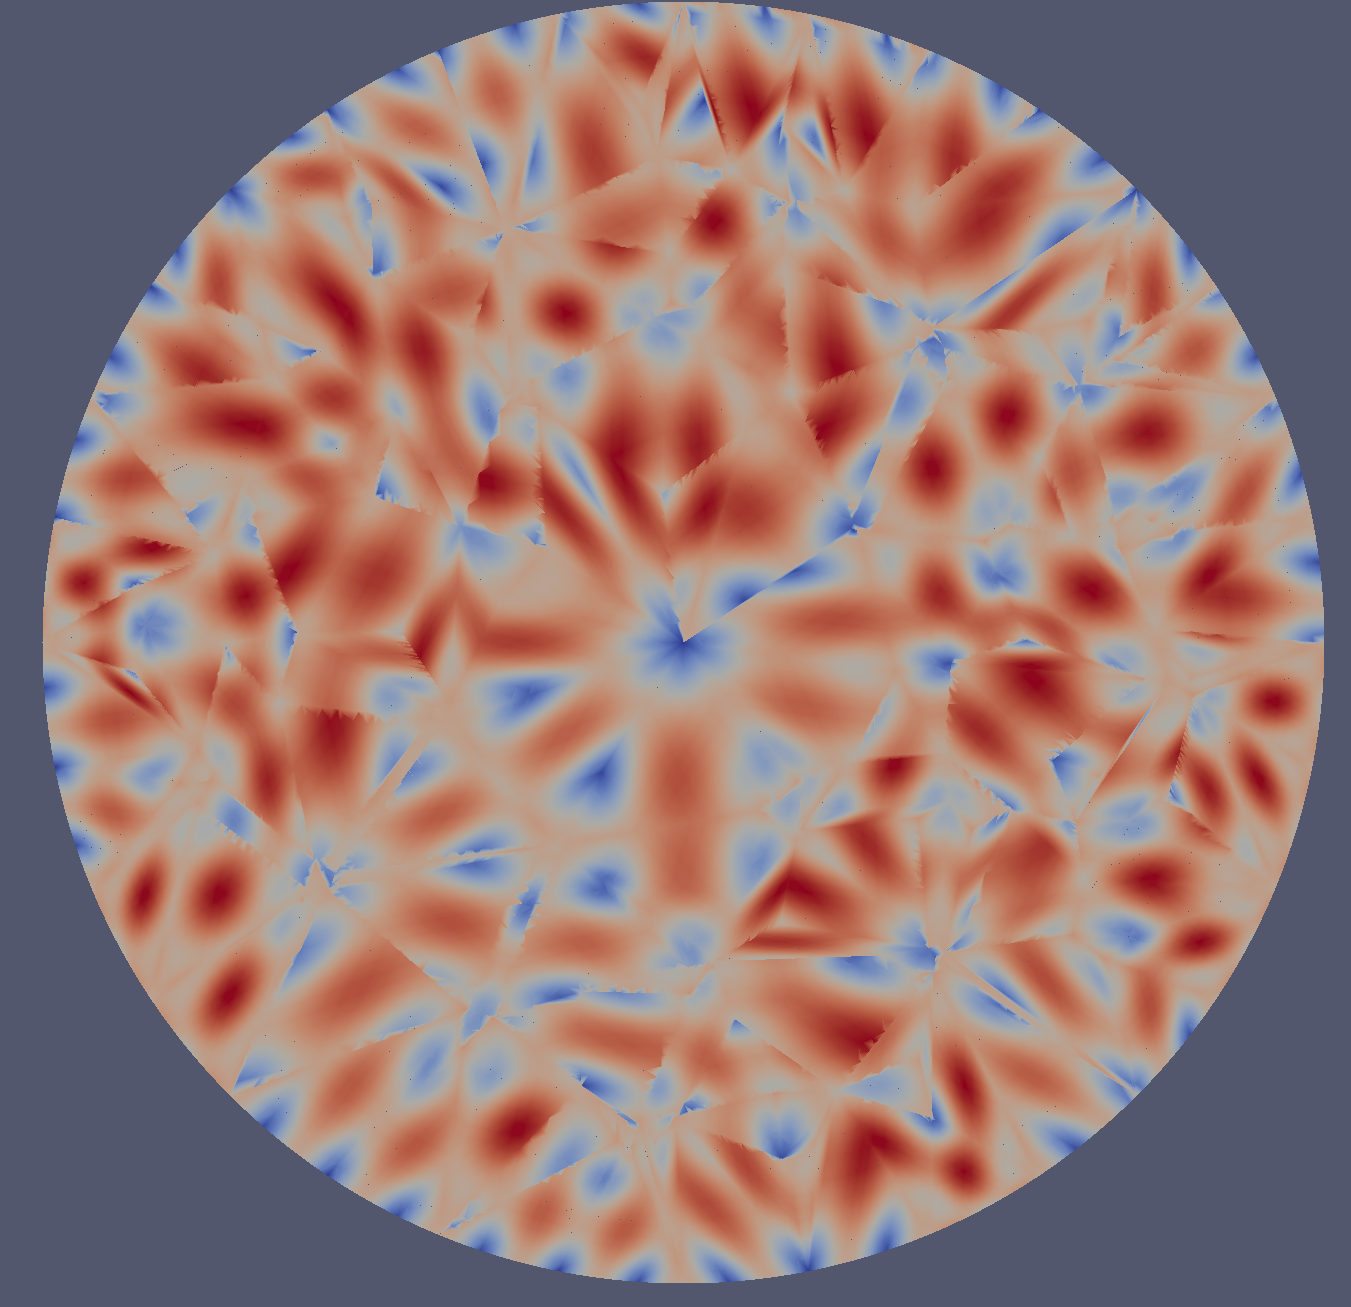
\includegraphics[scale=0.14]{images/tutorial3-vtk-localsinusoid} \end{subfigure}
	\begin{subfigure}[b]{0.45\textwidth} \hspace{4mm} 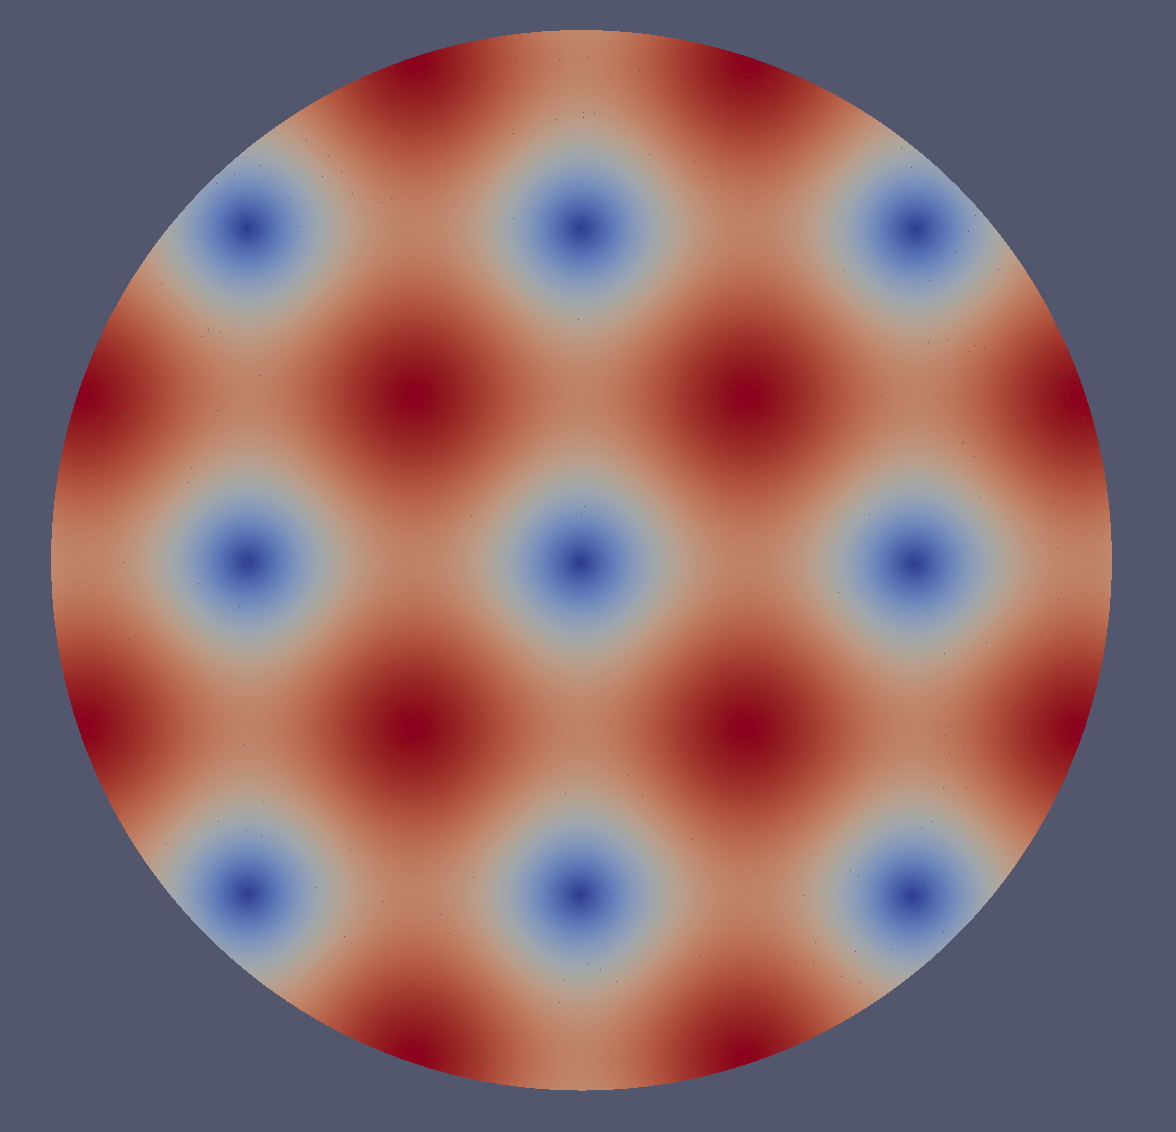
\includegraphics[scale=0.16]{images/tutorial3-vtk-globalsinusoid} \end{subfigure}
	\caption{ Visualization of tutorial 3. A sinusoid as function of local and global coordinates. This example emphasizes that there is no a priori orientation of the local coordinates. It is the task of the user to ensure that the local field is correctly oriented by considering the global indices of intersecting entities.}
	\label{fig:tutorial3:sinusoid}
\end{figure}


\subsection{Tutorial 4 - Quadrature Integration Tutorials}
\label{usage-howto-tutorial-integration-quadrature}

The following two tutorials demonstrate the capability of \curvgrid{} to address mathematical and physical problems requiring integration of certain quantities over the grid domain. \\


\noindent
\textbf{Scalar Surface Integral - \textit{Gauss} Law} \\
%
\noindent
In this example we verify \textit{Gauss} law numerically by computing the surface integral of the electric field produced by a unit point charge across the domain boundary of the mesh enclosing that charge. The tutorial will demonstrate that changing the curvature of the domain boundary or the position of the charge inside the domain does not affect the result that is $4 \pi$. More precisely, we compute the integral
\[\int_{\delta \Omega} \vec{E}(\vec{x}) \cdot d\vec{S} = \int_{\delta \Omega} \vec{E}(\vec{x}(\vec{u})) \cdot \vec{n}(\vec{u}) I(\vec{u}) d^2 u \]
\noindent
where $\vec{x}$ is the global coordinate, $\vec{u}$ is the coordinate local to the surface finite element,
\[\vec{E}(\vec{x}) = \frac{\vec{x} - \vec{x}_0}{|\vec{x} - \vec{x}_0|^{-3}}\]
is the electric field of a unit charge located at $\vec{x}_0$, $\vec{n}(\vec{u})$ is the surface outer normal in global coordinates as a function of local coordinates and
\[I(\vec{u}) = \sqrt{\det [ J^T(\vec{u}) J(\vec{u}) ]}\]
is the generalized integration element due to conversion of the integral from global to local coordinates (see \cref{appendix:integrationelements:proof}). \\

\noindent
In order to use the \curvgeom{} integration capabilities, the user must provide the integrand in the form of a functor class. The functor need not be overloaded, but must implement the $()$ operator

\begin{mybox}
\begin{lstlisting}
  ResultType operator()(const LocalCoordinate & x) const {...}
\end{lstlisting}
\end{mybox}

\noindent
as a function of the coordinate local to the entity it is evaluated over, in this case, a 2D coordinate local to a face. The code then iterates over all domain boundaries of the grid, calculating integrals of the functor over each boundary segment and adding up the results. In order to integrate a functor, the \textit{QuadratureIntegrator} class needs to be provided with the entity geometry, the functor to be integrated, the relative and absolute tolerances to be used for integration, as well as the norm type to be used for the case of multidimensional integration. 
\begin{mybox}
\begin{lstlisting}
  typedef Dune::QuadratureIntegrator<ct, DIM2D>  Integrator2DScalar;
  typedef typename Integrator2DScalar::template Traits<Integrand2D>::StatInfo  StatInfo;	
  StatInfo thisIntegralG = Integrator2DScalar::template integrateRecursive<FaceGeometry, Integrand2D, NORM_TYPE>(geometry, gaussf, RELATIVE_TOLERANCE, ACCURACY_GOAL);
\end{lstlisting}
\end{mybox}

\noindent
\textit{StatInfo} is the return data type of the \textit{QuadratureIntegrator}, which is a pair of the integral result and the quadrature order at which the desired relative accuracy was achieved. Note that the absolute accuracy \textit{ACCURACY\_GOAL} is used to determine if the integral is close enough to 0, as relative accuracy can not be used for this purpose due to division by 0. \\



\noindent
\textbf{Surface Vector Integral - Normal Integral} \\
%
\noindent
This test demonstrates the capability of \textit{QuadratureIntegrator} to integrate vector quantities. It tests the well-known identity, stating that the integral over the unit outer normal over a closed bounded domain is 0.

\begin{equation}
	\oiint_{\partial \Omega} n_x dS = \oiint_{\partial \Omega} \vec{e}_x \cdot \vec{n} dS = \iiint_{\Omega} \nabla \cdot \vec{e}_x dV = 0
\end{equation}

\noindent
The implementation of this test is almost identical to the \textit{Gauss} integral test above. The only difference is that \textit{Dune::FieldVector} is used as a functor output, and internally, instead of taking the dot product between the outer normal and the electric field, the normal itself is returned


%\subsection{Tutorial 4 - Recursive Numerical Integration}
%\label{usage-howto-tutorial-integration-recursive}


\subsection{Tutorial 5 - Communication via the DataHandle Interface}
\label{usage-howto-tutorial-communication}

This tutorial, consisting of two parts, serves as a simple use-case of interprocessor communication through grid entities, which is achieved via the \textit{DataHandle} interface. \\

\noindent
In the first tutorial we explicitly select all entities of the grid that are supposed to communicate for each available communication protocol, and communicate a dummy constant. The goal is to confirm that all the expected entities were communicated over, and all others were not. In the second tutorial, the global index of each entity is sent according to the specified communication protocol, and compared to the global index on the receiving side. It is demonstrated that these indices match for each communicating pair, and an exception is thrown should this not be the case. \\

% \noindent
% Briefly, the procedure communicateConstant iterates over all process process boundary intersections, and marks its neighbour entities, if they will be sending or receiving within the provided interface. Then the custom DataHandleConst is used to perform the communication. This data handle communicates one and the same constant to all entities it is requested. The important thing is that whenever gather or scatter methods are called, it checks if the requested entity was marked for sending or receiving, and throws an error if it is not. Finally, the main procedure checks that the total number of entities that have received the constant is equal to the number of entities marked for receiving.

\noindent
\curvgrid{} implements the \textit{DataHandle} communicators in accordance to the standard \dune{} interface, and its functionality does not exceed that envisioned by the standard interface. Since these tutorials are rather involved, and the standard mechanism is well-documented within the standard \dune{} reference, the detailed explanation of these two tutorials is beyond the scope of this paper. For further information, the user is referred to the \textit{Dune Grid Howto} documentation, found in \url{www.dune-project.org}



\subsection{Tutorial 6 - Parallel Data Output}

This tutorial demonstrates the use of a small utility \textit{ParallelDataWriter} designed for sorted parallel output of vectors. It explores the benefits of using the global element index provided by the mesh, for debugging of parallel numerical codes. The tutorial demonstrate that a quantity sampled over all elements of the grid and sorted by the element global index is independent of the number of processes used. Thus, the user can directly compare the output file, generated by runs with varying process count. \\

\noindent
\textit{Important Note: This tutorial only works if the mesh-provided global element index is re-used by the curvilinear \gmsh{} reader (default). If this is not the case, the automatically generated global index will depend on the number of processes and destroy the above symmetry.}

\noindent
This tutorial samples the volume of the elements. However, the interface of the \textit{ParallelDataWriter} extends to writing vectors of data for each element as well. One must first define the class

\begin{mybox}
\begin{lstlisting}
  <class Grid, class IndexType, class DataType>
  class ParallelDataWriter
\end{lstlisting}
\end{mybox}

\noindent
where \textit{IndexType} and \textit{DataType} are the data types of index and data arrays respectively. They can be any of the Plain Old Datatype (POD) classes, as long as their size is fixed over all processes for the communication purposes. One would then proceed to call the writer routine

\begin{mybox}
\begin{lstlisting}
  static void writeParallelData2File(std::string filename, std::vector<IndexType> & interiorElementGlobalIndex, std::vector<int> & interiorElementNDof, std::vector<DataType> & data, const Grid & grid)
\end{lstlisting}
\end{mybox}

\noindent
where \textit{interiorElementNDof} denotes the number of data entries per global index, and \textit{data} stores all data entries for all global indices in a contiguous 1D vector. \\


\subsection{Tutorial 7 - Global Boundary Communicator}

\noindent
This tutorial demonstrates the capabilities of \curvgrid{} to handle dense boundary communication problems, such as the Boundary Integral (BI) method. In the BI method, the global matrix or part of it correspond to pairwise coupling of every two faces on a given closed surface, providing a fully populated, i.e. dense, matrix. Each processor needs to obtain complete information of all faces on a given surface, collected over all processes.

\begin{mybox}
\begin{lstlisting}
  typedef Dune::CurvGrid::GlobalBoundaryContainer<GridType> BoundaryContainer;
  BoundaryContainer container(*grid, isDomainBoundary, volumeTag, surfaceTag);
\end{lstlisting}
\end{mybox}

\noindent
In case \textit{isDomainBoundary} is set to true, the \textit{BoundaryContainer} does not require the last two parameters. Otherwise, one must specify the surface tag of the interior surface, as well as the volume tag of elements either on the interior or the exterior of the surface, all one or the other. The unit outer normal for each face of the surface is determined as the unit outer normal of the associated element. Thus, if one provides the volume tag of the elements on the outside of the interior surface, one will always receive the inner unit normal at a later stage, and will have to multiply all of them by -1 in order to obtain the unit outer normal. The \textit{BoundaryContainer} does not contain the surfaces already located on this process, in order to save space.  \\

\noindent
In order to iterate over the \textit{BoundaryContainer}, we implement the accompanying \textit{BoundaryIterator}

\begin{mybox}
\begin{lstlisting}
  BoundaryIterator iter(container);
  while (!container.end()) {...}
\end{lstlisting}
\end{mybox}

\noindent
The boundary iterator re-implements most of the functionality of the standard Dune iterator, such as \textit{geometry()}, \textit{unitOuterNormal()}, \textit{indexInInside()}, \textit{geometryInInside()}, as well as some additional functionality compactified into the same iterator to save on communication complexity, such as 

\begin{mybox}
\begin{lstlisting}
  template <int codim>
  UInt globalIndex(UInt subIndexInFace) const {...}

  template <int codim>
  UInt globalIndexInParent(UInt subIndexInElem) const 

  UInt order() const { }

  BaseGeometryEdge geometryEdge(UInt subIndex) const {..}
\end{lstlisting}
\end{mybox}

\noindent
The tutorial performs several tests of the communicated boundary, such as the normal integral from Tutorial 4, calculation of total number of edges, as well as the complementarity of the global index of boundary surfaces located on this process, and on the \textit{BoundaryContainer}. \\




\subsection{Tutorial 8 - Interior Boundary}

The last tutorial extends the \textit{Gaussian} integral tutorial to interior boundaries, performing integrals for a set of charges inside and outside of the boundary. This is a simple test to verify if the interior boundary of the mesh forms a closed surface.


%%\subsection{Tutorial 5 - Polynomial Manipulation and Integration}
%%\label{usage-howto-tutorial-polynomial}
%%
%%
%%\subsection{Tutorial 7 - Point Location - OCTree}
%%\label{usage-howto-tutorial-octree}













%%%%%%%%%%%%%%%%%%%%%%%%%%%%%%%%%%%%%%%%%%%%%%%%%%%%%%%%%%%%%%%%%%%%%
% Curvilinear Grid Diagnostics - Section on mesh statistics and visualisation
%%%%%%%%%%%%%%%%%%%%%%%%%%%%%%%%%%%%%%%%%%%%%%%%%%%%%%%%%%%%%%%%%%%%%

%%\section{Diagnostics tools}
\subsection{Mesh statistics}
\subsection{Visualisation}



\chapter{Testing}







%%\newpage
%%\section{Interface - Curvilinear Geometry}

%%%%%%%%%%%%%%%%%%%%%%%%%%%%%%%%%%%%%%%
% Implementation of Interpolator Class
%%%%%%%%%%%%%%%%%%%%%%%%%%%%%%%%%%%%%%%
%%\section{Polynomial Interpolator Class}

\subsection{Methods}

\begin{itemize}
	\item \uline{Initialization:} Requires reference element/GeometryType, interpolatory vertex vector and interpolation order
	\item \uline{dofPerOrder:} Number of interpolatory vertices required for a given element type, dimension and interpolation order. For a simplex this quantity is
	\[ {DoF}_{dim}^{ord} = \{ \{ 2,3,4,5,6 \}, \{ 3,6,10,15,21 \}, \{ 4,10,20,35,56 \} \} \]
	\item \uline{cornerID:} The id number of a corner in the interpolatory vertex vector. For the simplices is calculated as follows:
		\subitem -for edge $\{ 0, \; ord \}$
		\subitem -for triangle $\{0, \; ord, \; {DoF}_{dim}^{ord} - 1\}$
		\subitem -for tetrahedron $\{0, \; ord, \; ord (ord + 3) / 2, \; {DoF}_{dim}^{ord} - 1\}$
	\item \uline{simplexGrid:} These 3 methods implement the functionality discussed in section \ref{subsection-simplexgrid}. They return a vector of indices which the grid points take in the d-dimensional matrix, and that vector divided by the interpolation order, which is exactly the local coordinates of the reference simplex grid.
	\item \uline{lagrangePolynomial:} Evaluates the i-th Lagrange Polynomial $L_i(\vec{r})$ for a given $i$ and a given local coordinate. Lagrange polynomials in this case are given explicitly for all orders to accellerate computation.
	\item \uline{realCoordinate:} Evaluates the global coordinate given a local coordinate. Computes the scalar product $\vec{p}(\vec{r}) = \sum_i \vec{p}_i L_i (\vec{r})$.
	\item \uline{interpolatoryVectorAnalytical:} Produces an analytical map from local to global coordinates in terms of polynomial vector.
		\subitem 0) Constructs local grid points $\vec{r}_i$ as given in \ref{subsection-simplexgrid}.		
		\subitem 1) Constructs monomial basis $\vec{z}^{ord}(\vec{r})$ as given in the beginning of section \ref{section-interppoly}
		\subitem 2) Evaluates all monomials $\vec{z}^{ord}(\vec{r})$ at all local grid points $\vec{r}_i$, assembling the DynamicMatrix V
		\subitem 3) Computes all lagrange polynomials using $\vec{L}(\vec{r}) = V^{-1} \vec{z}^{ord}(\vec{r})$
		\subitem 4) Computes the analytical map $\vec{p}(\vec{r}) = \sum_i \vec{p}_i L_i (\vec{r})$.
	\item \uline{SubentityInterpolators} Constructs Interpolator classes for each $\dim - 1$ subentity of the given element. Only allowed for elements of dimensions 2 and 3.
		\subitem - At the moment a rather crude algorithm is employed. To find the vertices corresponding to a given boundary, the order numbers of simplexGrid are written in a $(ord + 1) \times (ord + 1) \times (ord + 1)$ matrix, which is then used to easier locate the indices of the boundary interpolatory points in the vertex vector.
		\subitem - Certain orientation convention is chosen for the provided sub-entitiy interpolators, to simplify the future calculation of the outwards normals. The convention for edge orientations for a triangle $(012)$ are $(01)$, $(12)$ and $(20)$. The convention for triangle orientations for a tetrahedron $(0123)$ are $(012)$, $(023)$, $(213)$ and $(031)$.
\end{itemize}

\begin{figure}[hp]
    \centering
    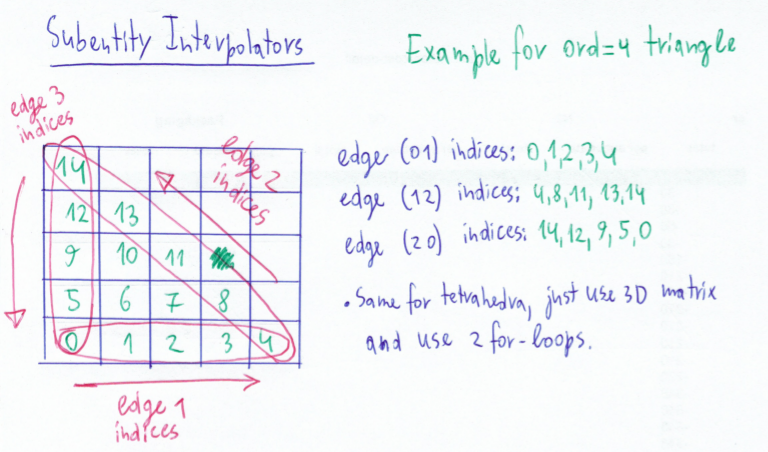
\includegraphics[scale=0.5]{doc-pics/pic-subentity-interpolators-method.png}
    %\caption{Awesome Image}
    %\label{fig:awesome_image}
\end{figure}


\subsection{Tests}

\noindent
For each dimension several linear and polynomial Functors are defined which act as pre-defined local-to-global maps. Then, for a simplex of each dimension there is a testing routine which is run for every applicable Functor. The tests are as follows:
\begin{itemize}
	\item For each order generate a local grid and sample the given functor to obtain global coordinates for interpolation points and thus construct the interpolator.
	\item First test requests a global coordinate for each local grid point, both using explicit function $realCoordinate$ and by evaluating the analytical polynomial provided by $interpolatoryVectorAnalytical$. Then the 3 results are compared. For this test, all 3 results must match independent of Functor and interpolation order.
	\item Second test requests a global coordinate for a random set of local coordinates, also comparing the correct result with explicit and analytical functionality. Explicit and analytical results should be equal to each other for any test since they do the same thing. However, they will match to the true result only if the polynomial order of the Functor is lower or equal to the one being tested, and most likely should fail for lower orders.
\end{itemize}

\textbf{TODO:}
\begin{itemize}
	\item The tests must be automatized such that the program throws an error if a test fails.
	\item Would be useful to test the method $SubentityInterpolators$ which is not tested at the moment, but is indirectly tested later in the LagrangeGeometry tests.
\end{itemize}


%%%%%%%%%%%%%%%%%%%%%%%%%%%%%%%%%%%%%%%
% Implementation of Recursive Integration
%%%%%%%%%%%%%%%%%%%%%%%%%%%%%%%%%%%%%%%
%%\section{Recursive Integrator Class}

Evaluates integral over element, approximating the integrand by an interpolatory polymomials of two hierarchical orders (2 and 4 at the moment). The running integration error is approximated by the difference between the analytical integrals calculated from these two interpolatory polynomials. The higher order element is split into into sub-elements of lower order, and the integration proceeds recursively. Every time an element is split, its previous running error is subtracted from the total error, and the running errors of the sub-elements are added to the total error. Thus, the integration is terminated when total approximated error is below selected tolerance. Heap structure ordered by the approximate error of the element is used to avoid recursion. At every iteration the element with the worst error is selected and then refined. When splitting, the previously calculated points are not re-calculated but hierarchically re-used by sub-elements. The sub-element only needs to be refined to a higher hierarchical order, by adding more points. \\

\noindent
\textit{Possible improvement - Performance}. As the the refined element does not check if the neighboring elements are also being refined, so they both sample on the boundary twice. Does there exist a method to store/find intersection refinements faster than just compute 2nd time. Using order 4 for every new refined triangle we sample 9 new points, out of which 2 are being wasted, thus $22\%$ inefficient.

\begin{figure}[p]
    \centering
    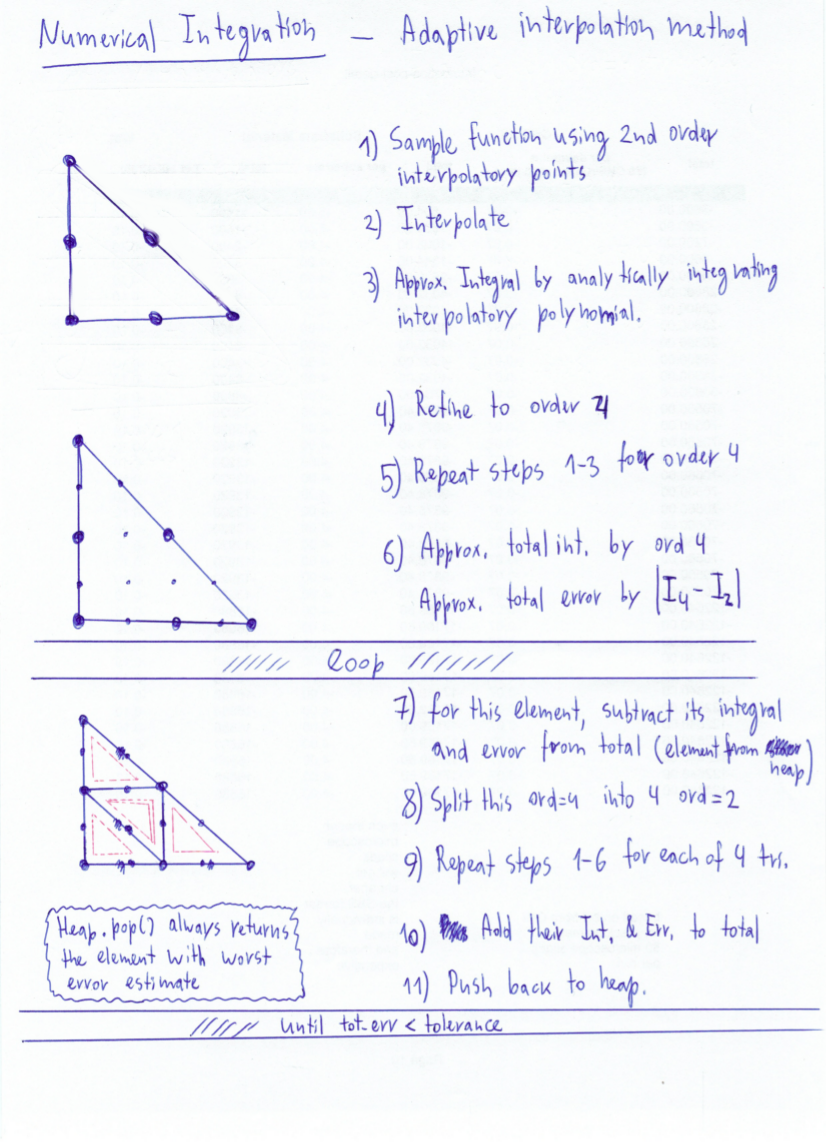
\includegraphics[scale=0.8]{doc-pics/pic-numerical-integration-adaptive-interpolation.png}
    %\caption{Awesome Image}
    %\label{fig:awesome_image}
\end{figure}


\subsection{Methods}

\noindent
Numerical Integration is only available for Simplices at the moment.

\noindent
\begin{itemize}
	\item \uline{Initialization:} Requires GeometryType to know the type of the element being integrated
	\item \uline{Integrate:} Integrates a function given by a functor object, until the expected integration error is below given tolerance.
\end{itemize}


\subsection{Tests}

\noindent
Numerical Integration is only implemented and hence tested for edges and triangles. A multitude of integrands are given in terms of Functors, starting with simple polynomial integrands and ending with integrands involving square roots of polynomials, as this is these are functions the method is expected to integrate well. The integrals are computed and compared to expected ones, which are sometimes given explicitly in numerical form, except of a lucky integral of $\iint \sqrt{xy} \; dxdy$ which happens to be $\pi / 24$. \\

\textbf{TODO:}
\begin{itemize}
	\item These tests should be automatized, which is easy to do, as they are only comparing numerical values.
	\item Integrals of complicated functions may exceed 100000 samples for this method given relative precision $10^{-5}$, which is too slow for the desired application
\end{itemize}


%%%%%%%%%%%%%%%%%%%%%%%%%%%%%%%%%%%%%%%
% Implementation of Recursive Integration
%%%%%%%%%%%%%%%%%%%%%%%%%%%%%%%%%%%%%%%
%%\section{Quadrature Integrator Class}
\label{interface-integrator-quadrature}

The Quadrature Integrator class provides static members to integrate functors over simplex reference elements by wrapping the quadrature rules provided by Dune. At the moment the dune-default Gauss-Legendre quadrature is used, however, the interface can be easily extended with flexibility to select the desired quadrature if need arises. The integrand functor must provide the operator \\

\begin{mybox}
\begin{lstlisting}
  double operator()(const Dune::FieldVector<ctype, mydim> & x)
\end{lstlisting}
\end{mybox}

\noindent
where $mydim$ must be equal to $gt.dim()$. Below 3 functions provide different strategies to approach integration \\

\begin{mybox}
\begin{lstlisting}
  template<class Functor>
  static ctype integrate(Dune::GeometryType gt, Functor f, int integrOrder)
  template<class Functor>
  static StatInfoVec integrateStat(Dune::GeometryType gt, Functor f, int integrOrderMax)
  template<class Functor>
  static StatInfo integrateRecursive(Dune::GeometryType gt, Functor f, ctype rel_tol)
\end{lstlisting}
\end{mybox}

\noindent
The first method integrates functor over the reference element using quadrature of a given order. The second method repeats the first method for all quadrature orders from 1 to specified maximal order, and outputs a vector of pairs (order, result). The last method integrates the functor with gradually increasing order until the desired estimated error tolerance is reached, or the maximal allowed quadrature order is reached. The estimated relative order is calculated as $\bigl | 1 - \frac{I(o)}{I_{smooth}(o-1)}  \bigr |$, where the smooth integral is defined as $I_{smooth}(o) = \zeta (I(o+1) + I(o-1)) + (1 - 2\zeta)I(o)$, with $\zeta$ being the smoothing parameter with default value $\zeta = 0.15$. The basic idea is to estimate the error as the difference between the integrals at consecutive orders.
\begin{itemize}
	\item Improvement 1: For some consecutive orders in Dune the number of quadrature points does not change, in this case simply skip to the next order.
	\item Improvement 2: Sometimes by random chance the two consecutive orders give very close results, while the integral still has not converged. To partially avoid this scenario, the smoothing parameter is introduced. The idea is to represent the previous best guess as a weighted average between a few previous estimates. So, if the integral has made a sharp jump recently, we will doubt that the integral has converged, thus the expected error will be larger.
\end{itemize}

\textbf{[TODO]}: To accelerate the gradual approximation strategy, it would be useful to implement a hierarchic quadrature. Such quadrature would double the interpolation order at every step, and reuse all the interpolation points already calculated.



%%%%%%%%%%%%%%%%%%%%%%%%%%%%%%%%%%%%%%%
% Implementation of Curvilinear Geometry
%%%%%%%%%%%%%%%%%%%%%%%%%%%%%%%%%%%%%%%
%%\subsection{Curvilinear Geometry Base Class}
\label{interface-curvilineargeometry}

\noindent
Curvilinear Geometry can be initialized either using the interpolator class, or the parameters necessary to initialize the interpolator class \\

\begin{mybox}
\begin{lstlisting}
  CurvilinearGeometry ( const ElementInterpolator & elemInterp)
  CurvilinearGeometry ( const ReferenceElement &refElement, const Vertices &vertices, InterpolatoryOrderType order)
  CurvilinearGeometry ( Dune::GeometryType gt, const Vertices &vertices, InterpolatoryOrderType order)
\end{lstlisting}
\end{mybox}

\noindent
Standard dune functionality \\
\begin{mybox}
\begin{lstlisting}
  bool affine ()
  GlobalCoordinate center ()
\end{lstlisting}
\end{mybox}

\noindent
Wrapper for basic interpolator functionality \\
\begin{mybox}
\begin{lstlisting}
  InterpolatoryOrderType order()
  Dune::GeometryType type()
  int nCorner ()
  int nVertex ()
  GlobalCoordinate corner ( InternalIndexType cornerLinearIndex )
  GlobalCoordinate vertex (int i)
  std::vector< GlobalCoordinate > cornerSet()
  std::vector<GlobalCoordinate> vertexSet()
\end{lstlisting}
\end{mybox}

\noindent
Wrapper for extended interpolator functionality \\
\begin{mybox}
\begin{lstlisting}
  ElementInterpolator interpolator()
  PolynomialVector interpolatoryVectorAnalytical()

  template<int subdim>
  CurvilinearGeometry< ctype, subdim, cdim>  subentityGeometry(InternalIndexType subentityIndex)
\end{lstlisting}
\end{mybox}

\noindent
Mappings \\
\begin{mybox}
\begin{lstlisting}
  GlobalCoordinate global ( const LocalCoordinate &local )
  bool local ( const GlobalCoordinate &globalC, LocalCoordinate & localC )
\end{lstlisting}
\end{mybox}

\noindent
Construction of normals \\
\begin{mybox}
\begin{lstlisting}
  GlobalCoordinate normal(const LocalCoordinate &local )
  GlobalCoordinate subentityNormal(InternalIndexType indexInInside, const LocalCoordinate &local )
  GlobalCoordinate subentityUnitNormal(InternalIndexType indexInInside, const LocalCoordinate &local )
  GlobalCoordinate subentityIntegrationNormal(InternalIndexType indexInInside, const LocalCoordinate &local )
\end{lstlisting}
\end{mybox}

%\noindent
%Construction numerical and analytic integration elements. \\

%\noindent
%\uline{JacobianDeterminantAnalytical}: $|\det J_{ij}|$ is available explicitly in polynomial form, when $(dim_{elem} = dim_{world})$. Although modulus is not a polynomial operation, $\det J_{ij} \neq 0$ inside the element, because the geometry must not be self-intersecting. Hence $\det J_{ij}$ is not allowed to change sign within the element, and modulus-correction is to evaluate $\det J_{ij}$ anywhere inside the element and multiply the analytic expression by $-1$ if the result is negative. \\

%\noindent
%\uline{NormalIntegrationElementAnalytical}: Surface normal integration element $d\vec{S} = \vec{n} dS $ is available. For edges in 2D defined by $d\vec{l} = (\partial_u p_y, -\partial_u p_x) du$. For triangles in 3D defined by $d \vec{S} = -(\partial_u \vec{p} \times \partial_v \vec{p}) du dv $ \\

%\noindent
%\uline{IntegrationElementSquaredAnalytical}: The square of the pseudodeterminant $\det(JJ^T)$, when $(dim_{elem} \neq dim_{world})$. For edges this expression is equal to $|\partial_u \vec{p}|^2$. For triangles in 3D this expression is equal to $|\vec{dS} / (du \; dv)|^2$. \\



\noindent
Numeric integration provided via standard integration elements, that can be further used in a quadrature routine. An exception to the interface is the volume method, which has do be done recursively, since the integration element need not be polynomial. Here, CurvilinearGeometry directly uses the recursive quadrature, and thus requires a tolerance parameter to terminate.

\begin{mybox}
\begin{lstlisting}
  ctype integrationElement ( const LocalCoordinate &local )
  JacobianTransposed jacobianTransposed ( const LocalCoordinate &local )
  JacobianInverseTransposed jacobianInverseTransposed ( const LocalCoordinate &local )
  ctype volume (double tolerance)
\end{lstlisting}
\end{mybox}




%\subsubsection{Methods - Cached Lagrange Geometry}
%\label{interface-curvilineargeometry-cached-methods}



\subsubsection{Tests}

\noindent
We start by explicitly defining the local-global mapping functors to mimic LagrangeGeometry for simplices of all 3 dimensions (Table 2). Then the following test procedure is run for each of the simplex mapping:
\begin{itemize}
	\item Loop over 5 interpolatory orders.
	\item For each order sample the interpolatory points from the mapping. Construct LagrangeGeometry and CurvilinearLagrangeGeometry classes.
	\item \textbf{Test 1}. To test if the Geometry has been correctly initialized, return all of its corners and check if they match those evaluated by the function.
	\item \textbf{Test 2}. To test local-to-global functionality, a random set of local points is sampled over the element, and the result of method $global()$ of the Geometry is compared with that of the explicit mapping. The test is omitted if the interpolation order is smaller than the order of the mapping.
	\item \textbf{Test 3}. To test global-to-local functionality, the local method is used for all the interpolation points expecting to obtain the points of the local interpolation grid over reference simplex. Also, it is checked if all these points are reported to be inside the element. This test fails a lot:
		\subitem -Fails to consider the point that is close to the boundary as in.
		\subitem -Fails to converge to a boundary point if the geometry has a zero derivative on the corner or on the whole boundary.
	\item \textbf{Test 4}. To test global-to-local using more probable sample points, the local coordinates are randomly sampled. It is then verified if $\vec{p} \approx local(global(\vec{p}))$. This test also checks if all the sample points are reported inside as they should be.
	\item \textbf{Test 5}. To check if the outside points are correctly sampled outside, as well as check the correctness of surface normal, we loop over all boundaries of the element, construct boundary normals for a uniform grid on the each boundary, and obtain the points which are just outside the element by calculating $\vec{p} = \vec{g} + \alpha \vec{n}$, where $\vec{g}$ is the global coordinate of of some point on the boundary, $\vec{n}$ is the normal at that point, and $\alpha = 0.01$ is a small number. \cref{fig:geometry:test:normal}.
	\item \textbf{Test 6}. The scalar basis functions given in Table 1 are integrated over the Geometry, and results are compared to those calculated by hand, given in Table 2.
	\item \textbf{Test 7}. The dot product surface integrals of vector basis functions (given in Table 3) over the Geometry are compared to those calculated by hand, given in Table 4.
\end{itemize}

\begin{figure}
    \centering
    
\includegraphics[scale=1.0]{images/normaltest}
	\captionsetup{width=0.8\textwidth} 
	\caption{ A combined test for normal accuracy and ability to accurately determine that a vertex is outside the element. Face normals sampled over a grid are used to produce global coordinates just outside the the element, which are then checked for having a local coordinate inside that element. }
	\label{fig:geometry:test:normal}
\end{figure}

\subsubsection{Integral-tests}

\begin{center}
\begin{tabular}{ | l | l | l |}
  \hline
  Ord & Dim & Scalar Basis Function \\ \hline
  0 & 1 & $1$ \\ \hline
  1 & 1 & $1 + 2x$ \\ \hline
  2 & 1 & $1 + 2x + 3x^2$ \\ \hline
  3 & 1 & $1 + 2x + 3x^2 + 4x^3$ \\ \hline
  4 & 1 & $1 + 2x + 3x^2 + 4x^3 + 5x^4$ \\ \hline
  5 & 1 & $1 + 2x + 3x^2 + 4x^3 + 5x^4 + 6x^5$ \\ \hline
%%  
  0 & 2 & $1$ \\ \hline
  1 & 2 & $1 + 2(x + y)$ \\ \hline
  2 & 2 & $1 + 2(x + y) + 3(x^2 + y^2) + xy$ \\ \hline
  3 & 2 & $1 + 2(x + y) + 3(x^2 + y^2) + xy + 4(x^3 + y^3) + xy^2$ \\ \hline
  4 & 2 & $\begin{array}{lcl} 1 & + & 2(x + y) + 3(x^2 + y^2) + xy + 4(x^3 + y^3) + xy^2 \\ & + & 5(x^4 + y^4) + xy^3 \end{array}$ \\ \hline
  5 & 2 & $\begin{array}{lcl} 1 & + & 2(x + y) + 3(x^2 + y^2) + xy + 4(x^3 + y^3) + xy^2 \\ & + & 5(x^4 + y^4) + xy^3 + 6(x^5 + y^5) + xy^4 \end{array}$ \\ \hline
%%  
  0 & 3 & $1$ \\ \hline
  1 & 3 & $1 + 2(x + y + z)$ \\ \hline
  2 & 3 & $1 + 2(x + y + z) + 3(x^2 + y^2 + z^2) + xy$ \\ \hline
  3 & 3 & $1 + 2(x + y + z) + 3(x^2 + y^2 + z^2) + xy + 4(x^3 + y^3 + z^3) + xyz$ \\ \hline
  4 & 3 & $\begin{array}{lcl} 1 & + & 2(x + y + z) + 3(x^2 + y^2 + z^2) + xy + 4(x^3 + y^3 + z^3) + xyz \\ & + & 5(x^4 + y^4 + z^4) + xyz^2 \end{array}$ \\ \hline
  5 & 3 & $\begin{array}{lcl} 1 & + & 2(x + y + z) + 3(x^2 + y^2 + z^2) + xy + 4(x^3 + y^3 + z^3) + xyz \\ & + & 5(x^4 + y^4 + z^4) + xyz^2 + 6(x^5 + y^5 + z^5) + xyz^3 \end{array}$ \\ \hline
\end{tabular}
\vfill
\title{Table 1. Scalar basis functions used, one of each polynomial order, one per geometry dimension}
\end{center}

\noindent
Using the vector basis functions $(x, x)$ for 2D edges and $(x, y, xy)$ for 3D triangles, we obtain the following integrals for the curvilinear maps

\begin{center}
\begin{tabular}{ | l | l | l | l | l | l | }
  \hline
  mydim & cdim & map               & Normal                  & Integrand                  & Result     \\ \hline
  1     & 2    & $(x,0)$           & $(0,-1)$                & $-x$                       & $-1/2$     \\ \hline
  1     & 2    & $(2x,3x)$         & $(3,-2)$                & $x$                        & $1/2$      \\ \hline
  1     & 2    & $(x,x^2)$         & $(2x,-1)$               & $2x^2-x$                   & $1/6$      \\ \hline
  2     & 3    & $(x,y,0)$         & $(0,0,-1)$              & $-xy$                      & $-1/24$    \\ \hline
  2     & 3    & $(y,3x,x+y)$      & $(-3,-1,3)$             & $-3x-y+3xy$                & $-13/24$   \\ \hline
  2     & 3    & $(y^2,x^2,xy)$    & $(-2y^2,-2x^2,4xy)$     & $-2x^3-2y^3+4x^2y^2$      & $-17/180$   \\ \hline
\end{tabular}
\\
\title{Table 3. DotProduct Integrals of Vector basis functions over curved boundaries}
\end{center}


\begin{landscape}

\begin{center}
\begin{tabular}{ | l | l | l | l | l | l | l | l | l |}
  \hline
  $d_e$ & Map & $\mu(\vec{r})$ & $I_0$ & $I_1$ & $I_2$ & $I_3$ & $I_4$ & $I_5$ \\ \hline
  1 & $(x)$                & $1$ & $1.0$ & $2.0$ & $3.0$ & $4.0$ & $5.0$ & $6.0$ \\ \hline
  1 & $(x,0)$              & $1$ & $1.0$ & $2.0$ & $3.0$ & $4.0$ & $5.0$ & $6.0$ \\ \hline
  1 & $(x,0,0)$            & $1$ & $1.0$ & $2.0$ & $3.0$ & $4.0$ & $5.0$ & $6.0$ \\ \hline
  1 & $(1+2x)$             & $2$ & $2.0$ & $4.0$ & $6.0$ & $8.0$ & $10.0$ & $12.0$ \\ \hline
  1 & $(2x,3x)$            & $\sqrt{13}$ & $\sqrt{13}$ & $2\sqrt{13}$ & $3\sqrt{13}$ & $4\sqrt{13}$ & $5\sqrt{13}$ & $6\sqrt{13}$ \\ \hline
  1 & $(2x,0.5+3x,5x)$     & $\sqrt{38}$ & $1\sqrt{38}$ & $2\sqrt{38}$ & $3\sqrt{38}$ & $4\sqrt{38}$ & $5\sqrt{38}$ & $6\sqrt{38}$ \\ \hline
  1 & $(x^2)$              & $2x$ & $1.0$ & $7/3$ & $23/6$ & $163/30$ & $71/10$ & $617/70$ \\ \hline
  1 & $(x,x^2)$            & $\sqrt{1 + 4x^2}$ & $1.47894286$ & $3.175666172$ & $4.994678155$ & $6.89140143$ & $8.84167808$ & $10.83102449$ \\ \hline
  1 & $(x,x^2,2)$          & $\sqrt{1 + 4x^2}$ & $1.47894286$ & $3.175666172$ & $4.994678155$ & $6.89140143$ & $8.84167808$ & $10.83102449$ \\ \hline
  2 & $(x,y)$              & $1$ & $1/2$ & $7/6$ & $41/24$ & $17/8$ & $37/15$ & $2.75714$ \\ \hline
  2 & $(x,y,0)$            & $1$ & $1/2$ & $7/6$ & $41/24$ & $17/8$ & $37/15$ & $2.75714$ \\ \hline
  2 & $(1+x,x+y)$          & $1$ & $1/2$ & $7/6$ & $41/24$ & $17/8$ & $37/15$ & $2.75714$ \\ \hline
  2 & $(y,3x,x+y)$         & $\sqrt{19}$ & $\sqrt{19}/2$ & $7\sqrt{19}/6$ & $41\sqrt{19}/24$ & $17\sqrt{19}/8$ & $37\sqrt{19}/15$ & $2.75714 \sqrt{19}$ \\ \hline
  2 & $(x^2,y^2)$          & $4xy$ & $1/6$ & $13/30$ & $59/90$ & $103/126$ & $0.94127$ & $1.03915$ \\ \hline
  2 & $(x^2,y^2,xy)$       & $2\sqrt{x^4+y^4+4x^2 y^2}$ & $0.360858$ & $0.938231$ & $1.47326$ & $1.93004$ & $2.33506$ & $2.70079$ \\ \hline
  3 & $(x,y,z)$            & $1$ & $1.0/6$ & $5.0/12$ & $23.0/40$ & $0.676389$ & $0.748214$ & $0.801935$ \\ \hline
  3 & $(x+y,y+z,x+z)$      & $2$ & $1.0/3$ & $5.0/6$ & $23.0/20$ & $2\cdot 0.676389$ & $2\cdot 0.748214$ & $2\cdot 0.801935$ \\ \hline
  3 & $(x^2,y^2,z^2)$      & $8xyz$ & $1.0/90$ & $0.0301587$ & $0.0416667$ & $0.0481922$ & $0.0522134$ & $0.05483$ \\ \hline
\end{tabular} \vfill
\title{Table 2. Explicit mappings for element curvatures, and the integrals of B.F. from Table 1}
\end{center}

\end{landscape}




%\newpage
%\section{Interface - Curvilinear Grid}

%%%%%%%%%%%%%%%%%%%%%%%%%%%%%%%%%%%%%%%
% Interface of Curvilinear Grid Factory
%%%%%%%%%%%%%%%%%%%%%%%%%%%%%%%%%%%%%%%
%%\section{Curvilinear Grid}
\label{interface-curvilineargrid}

This section will discuss the new methods available to the curvilinear grid, which extend the dune-grid interface.

%%\section{Curvilinear Grid Base Implementation}

%%%%%%%%%%%%%%%%%%%%%%%%%%%%%%%%%%%%%%%
% Interface of Curvilinear GMSH Reader
%%%%%%%%%%%%%%%%%%%%%%%%%%%%%%%%%%%%%%%
%%\subsection{Curvilinear GMSH Reader}
\label{interface-gmsh-reader}

This section will precisely discuss the access to the factory and GMSH Reader

\begin{mybox}
\begin{lstlisting}
    Dune::CurvilinearGmshReader< GridType >::read(factory, filename, mpihelper, verbose, processVerbose, writeReaderVTKFile, insertBoundarySegment); 
\end{lstlisting}
\end{mybox}


%%%%%%%%%%%%%%%%%%%%%%%%%%%%%%%%%%%%%%%
% Interface of Curvilinear VTK Writer
%%%%%%%%%%%%%%%%%%%%%%%%%%%%%%%%%%%%%%%
%%\section{Curvilinear VTK Writer}
\label{interface-vtk-writer}


This section will precisely discuss the VTK writer

\begin{mybox}
\begin{lstlisting}
  Dune::CurvilinearVTKWriter<GridType> vtkCurvWriter(verbose, processVerbose, mpihelper);
\end{lstlisting}
\end{mybox}

\begin{mybox}
\begin{lstlisting}
  std::vector<int> tags  { physicalTag, structType, mpihelper.rank() };
\end{lstlisting}
\end{mybox}

\begin{mybox}
\begin{lstlisting}
  vtkCurvWriter.template addCurvilinearElement<mydim>(gt, interpVertices, tags, interpOrder, N_DISCRETIZATION_POINTS, interpolate, explode, WRITE_VTK_EDGES, WRITE_VTK_TRIANGLES);
\end{lstlisting}
\end{mybox}








%%\section{Implementation Details}

%%%%%%%%%%%%%%%%%%%%%%%%%%%%%%%%%%%%%%%%%%%%%%%%%%%%%%%%%%%%%%%%%%%%%
% Implementation Details - Curvilinear Element Interpolator
%%%%%%%%%%%%%%%%%%%%%%%%%%%%%%%%%%%%%%%%%%%%%%%%%%%%%%%%%%%%%%%%%%%%%

%%\section{Implementation Details - Curvilinear Geometry}

\subsection{Local-to-global Mapping}

\subsection{Normals}

\subsection{Analytical Integration}










\appendix

\chapter{Proofs}

%%%%%%%%%%%%%%%%%%%%%%%%%%%%%%%%%%%%%%%
% Proof of explicit expression for the integration elements
%%%%%%%%%%%%%%%%%%%%%%%%%%%%%%%%%%%%%%%
\section{Integration Elements}

When transforming an integral over an entity from global to local coordinates, the resulting integral acquires an additional prefactor called Integration Element

\[ \int_{V} dx dy dz = \int_{V'} I(u,v,w) du dv dw \]

\noindent
\textbf{Edge(1D Local Coordinates)}:
\[\vec{dl} = \vec{p}(u + du) - \vec{p}(u) = \frac{\partial \vec{p}}{\partial u} du \]
\[dl = |\vec{dl}| = |\frac{\partial \vec{p}}{\partial u}| du = I(u)du \]
For example, if global coordinates are 3D, then
\[I(u) = \sqrt{\bigl (\frac{\partial x}{\partial u})^2 + \bigl (\frac{\partial y}{\partial u})^2 + \bigl (\frac{\partial z}{\partial u})^2} \]

\noindent
\textbf{Face(2D Local Coordinates)}:
\[\vec{dA} = (\vec{p}(u + du, v) - \vec{p}(u, v)) \times (\vec{p}(u, v + dv) - \vec{p}(u, v)) = \frac{\partial \vec{p}}{\partial u} \times \frac{\partial \vec{p}}{\partial v} du dv \]
\[dA = |\vec{dA}| = \bigl | \frac{\partial \vec{p}}{\partial u} \times \frac{\partial \vec{p}}{\partial v} \bigr | du dv \]
For example, if global coordinates are 3D, then
\[I(u,v) = \biggl | \begin{pmatrix}
  \partial_u y \partial_v z - \partial_u z \partial_v y \\
  \partial_u z \partial_v x - \partial_u x \partial_v z \\
  \partial_u x \partial_v y - \partial_u y \partial_v x
\end{pmatrix} \biggr | du dv \]

\noindent
\textbf{Element(3D Local Coordinates)}:
\begin{eqnarray*}
  dV & = & ((\vec{p}(u + du, v, w) - \vec{p}(u, v, w)) \times (\vec{p}(u, v + dv, w) - \vec{p}(u, v, w))) \\
     && \cdot  (\vec{p}(u, v + dv, w) - \vec{p}(u, v, w)) du dv dw  \\
     & = & (\partial_u \vec{p} \times \partial_v \vec{p}) \cdot \partial_w \vec{p} \; du dv dw
\end{eqnarray*}
\[ I(u,v,w) = (\partial_u \vec{p} \times \partial_v \vec{p}) \cdot \partial_w \vec{p} \]

\noindent
It can be shown that the three above cases can all be rewritten as
\[ I(\vec{r}) = \sqrt{\det(J(\vec{r})^T J(\vec{r}))} \]
where $\vec{r}$ are the local coordinates, and $J(\vec{r})$ is the Jacobian transformation defined as
\[J(\vec{r}) = \frac{\partial \vec{p}}{\partial \vec{r}}\]
which, for 3D global coordinates can be written as
\[J_{Edge}(u) = \bigl(\frac{\partial x}{\partial u}, \frac{\partial y}{\partial u}, \frac{\partial z}{\partial u} \bigr)  \]
\[J_{Face}(u,v) = 
\begin{pmatrix}
   \partial_u x &&    \partial_u y  &&    \partial_u z \\
   \partial_v x &&    \partial_v y  &&    \partial_v z
\end{pmatrix}
\]
\[J_{Elem}(u,v,w) = 
\begin{pmatrix}
   \partial_u x &&    \partial_u y  &&    \partial_u z \\
   \partial_v x &&    \partial_v y  &&    \partial_v z \\
   \partial_w x &&    \partial_w y  &&    \partial_w z
\end{pmatrix}
\]

\noindent
Finally, in case where local and global dimension matches (e.g. edge in 1D, face in 2D, element in 3D), the Jacobian is a square matrix. If the geometry is strictly non-singular ($\det{J} > 0$ everywhere within the entity), the general expression for the integration element can be simplified to
\[ I(\vec{r}) = \det{J(\vec{r})} \]

%%%%%%%%%%%%%%%%%%%%%%%%%%%%%%%%%%%%%%%
% Proof of polynomial integral over simplex
%%%%%%%%%%%%%%%%%%%%%%%%%%%%%%%%%%%%%%%
\subsection{Duffy Transform}
\label{section-abstract-duffy-transform}

The \textit{Duffy} transform is is a bijective map between the local coordinate of a hypercube and another entity, in our case, the reference simplex. Further, one can use the \textit{Duffy} transform to directly apply the hypercubic integration routines (e.g. tensor product quadrature rules) to simplex domains. Effectively, the \textit{Duffy} transform claims that
\[\int_{\triangle} f(\vec{x}) d\vec{x} = \int_{\Box} g(\vec{\tau}) f(\vec{x}(\vec{\tau})) d\vec{\tau},\]
giving explicit expressions for $g(\vec{\tau})$ and $\vec{x}(\vec{\tau})$. \\

\noindent
We consider simplices of all dimensions up to 3: \\

\noindent
\textbf{1D}: The reference hypercube and simplex are both an edge defined on $[0, 1]$, so they have exactly the same parameter. \\

\noindent
\textbf{2D}: Here we map from reference triangle to reference square. We transform the integral of interest, namely

\[ \int_0^1 \int_0^{1-x} f \biggl(
\begin{matrix}  x \\ y  \end{matrix} \biggr)
 dx dy = \int_0^1 \int_0^1 (1-x) 
f \biggl( \begin{matrix} x \\ (1-x)t \end{matrix} \biggr)
dx dt \]

\noindent
using a substitution $t = y / (1 - x)$, such that $t \in [0, 1]$. \\

\noindent
\textbf{3D}: Here we map from the reference tetrahedron to the reference cube. We transform the integral of interest, namely

\[ \int_0^1 \int_0^{1-x} \int_0^{1-x-y} f \scalebox{1.2}{\Bigg(}
\begin{matrix}  x \\ y \\ z  \end{matrix} \scalebox{1.2}{\Bigg)}
dx dy = \int_0^1 \int_0^1 \int_0^1 (1-x)^2 (1-t)
f \scalebox{1.2}{\Bigg(} \begin{matrix}  x \\ (1-x)t \\ (1-x)(1-t)\tau  \end{matrix} \scalebox{1.2}{\Bigg)}
dx dt d\tau \]

\noindent
using a substitution $t = \frac{y}{1 - x}, \tau = \frac{z}{(1 - x)(1 - t)}$, such that $t,\tau \in [0, 1]$. \\

%%%%%%%%%%%%%%%%%%%%%%%%%%%%%%%%%%%%%%%
% Method of dealing with first order singular integrals
%%%%%%%%%%%%%%%%%%%%%%%%%%%%%%%%%%%%%%%
%% \section{Singularity Elimination}

\subsection{First order scalar integral}
\label{appendix-singularity-1st-scalar}

When implementing surface integral methods, one has to deal with singular integrals over the face of the element, which take the form
\[ \iint \frac{g(x,y)}{|\vec{x} - \vec{x}_0|} dx dy \]
where $g(x,y)$ is analytic. Principal value integration has to be used to analytically determine the value of the integral within the infinitesimal area patch including the singularity.
This is beyond the scope of the current section. Instead, we assume that the contribution of the singularity has already been considered. What remains is to develop a procedure to
numerically compute the remainder of the integral, eliminating the singularity and avoiding numerical instabilities. \\

\noindent
\textbf{[CITEDUFFY]} propose a method to eliminate the singularity for integrals over a reference triangle. Consider the integral over a reference triangle
\[ \int_0^1 \int_0^{1-x} \frac{g(x,y)}{|\vec{x} - \vec{x}_0|} dx dy \]
It is proposed to first deal with the special case $\vec{x}_0 = (1,0)$, that is, having the singularity in the bottom-right corner of the reference triangle.
Thus, the integral can be simplified to
\[ \int_0^1 \int_0^{1-x} \frac{g(x,y)}{\sqrt{(x-1)^2 + y^2}} dx dy \]
By changing the variable of the $y$-integral to $y=(1-x)t$, we get
\[ \int_0^1 \int_0^1 \frac{g(x,(1-x)t)}{\sqrt{(x-1)^2 + t^2(1-x)^2}} (1-x)dx dt \]
Since the contribution of the singularity itself is assumed to have already been accounted for, we may divide the numerator and denominator by $(1-x)$, ignoring the case $0/0$.
Thus, we have transformed an integral over a reference triangle to equivalent integral over a reference square
\[ \int_0^1 \int_0^1 \frac{g(x,(1-x)t)}{\sqrt{1 + t^2}} dx dt \]
which does not have a singularity, and can thus easily be integrated using your favourite quadrature.

\noindent
Now we need to generalize the above method to deal with all the singularities except $\vec{x}_0 = (1,0)$. This can be accomplished by subdividing the existing triangle
into (at most) 3 smaller triangles, for each of which the singularity is at the desired corner \textbf{[PICHERE]}. Thus, for each triangle we will construct a linear
mapping $(u,v) = \psi(u', v')$, where $(u', v')$ are the local coordinates of the sub-triangle. \\

\noindent
The problem is that the coordinate transformation slightly changes the form of the denominator, requiring us to adapt our procedure. In addition, the singularity is frequently given
in terms of the global coordinates, obtained, in general, using the curvilinear mapping $\vec{x} = \vec{p}(u, v)$. Considering both of these generalizations, we can write the more general
form of the singular integral as 
\[ \int_0^1 \int_0^{1-u'} \frac{g(u',v')}{|\vec{p}(\vec{\psi}(\vec{r}')) - \vec{p}(\vec{\psi}(\vec{r}_0'))|} du' dv' \]
where $\vec{r}' = (u', v')$ are the local coordinates of the sub-triangle. To simplify this equation, we can design a general polynomial mapping $p' = p \circ \psi$.
Since both maps are polynomial, the resulting map is obtained by substituting one polynomial into another.

\noindent
We use the same Duffy transform $v' = (1-u')t$ to obtain an integral over the reference square
\[ \int_0^1 \int_0^1 \frac{g(u',(1-u')t)}{|\vec{p}'(u',(1-u')t) - \vec{p}'(\vec{r}_0')|} (1-u')du' dt \]
Now let us consider, what happens to the denominator, if we choose the singularity to still be at the corner $\vec{r}_0' = (1,0)$.
The denominator $|\vec{p}'(u',(1-u')t) - \vec{p}'(1,0)|$, which is a polynomial, is clearly divisible by $(1-u')$, because $u' = 1$ is its solution. Again, we will divide the denominator
and numerator by $(1-u')$, eliminating the singularity, and obtaining the integral
\[ \int_0^1 \int_0^1 \frac{g(u',(1-u')t)}{|\vec{\zeta}(u', t)|} du' dt \]
All that remains is to find the explicit form of $\vec{\zeta}(u', t)$. By looping over all monomial summands of $\vec{p}'(u',v')$, we can rewrite it by splitting it into terms that
are proportional to $v'$ and terms that are not. For all the terms that are proportional to $v'$, we will bring one instance of $v'$ in front of the sum
\[ \vec{p}' = \vec{p}'(u', 0) + v' R(u', v') = \vec{p}'(u', 0) + (1-u')t R(u', v') \]
Thus, after division by $(1-u')$, we get
\[ \vec{\zeta} = \frac{\vec{p}'(u', 0) - \vec{p}'(1, 0)}{1-u'} + t R(u', v') \]
Finally, the division in the first fraction can be performed by considering that the numerator is a 1D polynomial of the form $\sum_{i \geq 1} a_i (x^i - 1)$.
Each monomial separately can be divided by $(1-u')$ by considering the identity
\[ \frac{x^n - 1}{x - 1} = \sum_{i=0}^{n-1} x^i \]


\textbf{[TODO]}
\begin{itemize}
  \item Show that resulting polynomial integral is not singular
  \item What to do with integrals over neighbouring elements
\end{itemize}






\subsection{First order vector integral}
\label{appendix-singularity-1st-vector}

A slightly more sophisticated integral has 2nd order singularity in the denominator, but is proportional to the vector distance, and this can be made use of

\[ \int_0^1 \int_0^{1-u'} \frac{g(u',v') (\vec{p}(\vec{r}) - \vec{p}(\vec{r}_0))}{|\vec{p}(\vec{r}) - \vec{p}(\vec{r}_0)|^2} du' dv' \]

\noindent
Following exactly the steps in \cref{appendix-singularity-1st-scalar}, one denominator order will be absorbed by the coordinate transform, and the other by the vector distance, resulting in the equation

\[ \int_0^1 \int_0^1 \frac{g(u',(1-u')t) \vec{\zeta}(u', t)}{|\vec{\zeta}(u', t)|^2} du' dt \]





\subsection{Second and higher order vector integrals}

The most sophisticated integral we will treat is 

\[ \int_0^1 \int_0^{1-u'} \frac{g(u',v') (\vec{p}(\vec{r}) - \vec{p}(\vec{r}_0))}{|\vec{p}(\vec{r}) - \vec{p}(\vec{r}_0)|^n} du' dv' \]
\noindent
where $n \geq 3$. Performing the steps from \cref{appendix-singularity-1st-vector}, we obtain 
\[ \int_0^1 \int_0^1 \frac{g(u',(1-u')t) \vec{\zeta}(u', t)}{|\vec{\zeta}(u', t)|^n (u' - 1)^{n-2}} du' dt \]
\noindent
thus having "softened" the singularity by by one order of magnitude, and removed the vectorial dependence. The problem has now been converted to a 1D problem of the type

\[ \int_0^1 \frac{F(u)}{(1-u)^{n-2}}du  \]







%%%%%%%%%%%%%%%%%%%%%%%%%%%%%%%%%%%%%%%
% Proof of polynomial integral over simplex
%%%%%%%%%%%%%%%%%%%%%%%%%%%%%%%%%%%%%%%
\section{Proof for polynomial summand integrals}
\label{appendix-proof-simplexintegral}


\noindent
Note that the series for beta-function can be written as
\[B(a+1,b+1) = \int_0^1 x^a (1-x)^b dx = \int_0^1 x^a \sum_{i=0}^b C_b^i (-1)^i x^i = \sum_{i=0}^b \frac{(-1)^i C_b^i}{a+1+i}\]

\noindent
where $C_b^i = \frac{b!}{i!(b-i)!}$ is the combinations number. \\

\noindent
\textbf{1D:} \\

\begin{equation}
	I_{1D} = \int_0^1 x^{\alpha} dx = \frac{x^{a + 1}}{a + 1} \biggr |_0^1 = \frac{1}{a + 1}
\end{equation}

\noindent
\textbf{2D:} \\

\begin{eqnarray*}
	I_{2D} = \int_0^1 \int_0^{1-x} x^{a} y^{b} dx dy
	& = & \frac{1}{b+1} \int_0^1 x^{a} (1-x)^{b+1} dx = \frac{1}{b+1} \beta(a + 1, b + 2) \\
	& = & \frac{1}{b+1} \frac{a!(b+1)!}{(a+b+2)!} = \frac{a!b!}{(a+b+2)!}
\end{eqnarray*}

\noindent
\textbf{3D:} \\

\begin{eqnarray*}
	I_{3D}
	& = & \int_0^1 \int_0^{1-x} \int_0^{1-x-y} x^a y^b z^c dx dy dz \\
	& = & \frac{1}{c+1} \int_0^1 \int_0^{1-x} x^a y^b (1-x-y)^{c+1} dx dy \\
	& = & \frac{1}{c+1} \int_0^1 \int_0^{1-x} x^a y^b \sum_{i=0}^{c+1} C_{c+1}^i (-1)^i y^i (1-x)^{c+1-i} dx dy \\
	& = & \sum_{i=0}^{c+1} \frac{C_{c+1}^i (-1)^i}{c+1} \int_0^1 \ x^a (1-x)^{c+1-i} \int_0^{1-x} y^{b+i} dx dy \\
	& = & \sum_{i=0}^{c+1} \frac{C_{c+1}^i (-1)^i}{(c+1)(b+1+i)} \int_0^1 \ x^a (1-x)^{c+1-i} (1-x)^{b+1+i} dx \\
	& = & \sum_{i=0}^{c+1} \frac{C_{c+1}^i (-1)^i}{(c+1)(b+1+i)} \int_0^1 \ x^a (1-x)^{b+c+2} dx \\
	& = & \sum_{i=0}^{c+1} \frac{C_{c+1}^i (-1)^i}{(c+1)(b+1+i)} \beta(a+1, b+c+3) \\
	& = & \frac{1}{c+1} \beta(b+1,c+2) \beta(a+1, b+c+3) \\
	& = & \frac{1}{c+1} \frac{b!(c+1)!}{(b+c+2)!} \frac{a! (b+c+2)!}{(a+b+c+3)!} \\
	& = &  \frac{a! b! c!}{(a+b+c+3)!}
\end{eqnarray*}


\chapter{Interfaces}

%%%%%%%%%%%%%%%%%%%%%%%%%%%%%%%%%%%%%%%
% Implementation of Polynomial Class
%%%%%%%%%%%%%%%%%%%%%%%%%%%%%%%%%%%%%%%
\subsection{Polynomial Class}
\label{interface-geometry-polynomial}

\noindent
An arbitrary polynomial of order $n$ with $d$ parameters can be represented in its expanded form as
\[ p(\vec{u}) = \sum_i A_i \prod_{j = 0}^d u_j^{\mathrm{pow}_{i,j}},  \]
where ${pow}_{i,j}$ is the power $j$\textsuperscript{th} dimension of $i$\textsuperscript{th} summand. For example, in 3D this can be written as
\[ p(\vec{u}) = \sum_i A_i u^{pow_{u,i}} v^{pow_{v,i}} w^{pow_{w, i}},  \]

\noindent
We define a Monomial class, which stores a constant multiplier $A$ and vector of powers $pow$. \\

\begin{mybox}
\begin{lstlisting}
  PolynomialTraits::Monomial(double prefNew, std::vector<int> powerNew)
\end{lstlisting}
\end{mybox}

\noindent
A polynomial can be constructed either empty, from a single monomial or from another polynomial. \\

\begin{mybox}
\begin{lstlisting}
  Polynomial()
  Polynomial(Monomial M)
  Polynomial(const Polynomial & other)
\end{lstlisting}
\end{mybox}

\noindent
The below interface provides methods to perform basic algebraic operations with polynomials and scalars. The method $axpy$ is the scaled addition, equivalent to $this += other * a$ \\

\begin{mybox}
\begin{lstlisting}
  LocalPolynomial & operator+=(const Monomial & otherM)
  LocalPolynomial & operator+=(const LocalPolynomial & other)
  LocalPolynomial & operator*=(const double c)  
  LocalPolynomial & operator*=(const LocalPolynomial & other)  
  void axpy(LocalPolynomial other, double c)
  LocalPolynomial operator+(const LocalPolynomial & other)
  LocalPolynomial operator+(const ctype a)  
  LocalPolynomial operator-(const LocalPolynomial & other)  
  LocalPolynomial operator-(const ctype a)  
  LocalPolynomial operator*(const ctype a)  
  LocalPolynomial operator*(const LocalPolynomial & other)
\end{lstlisting}
\end{mybox}

\noindent
We have implemented differentiation, integration and evaluation a polynomials. $derivative$ routine returns the partial derivative of a polynomial w.r.t. coordinate indexed by the parameter; $evaluate$ routine evaluates the polynomial at the provided local coordinate; $integrateRefSimplex$ routine integrates the polynomial over the reference entity of the same dimension as the polynomial, returning a scalar. An integral of a monomial over the reference simplex has an analytical expression, see \ref{appendix-proof-simplexintegral} \\


\begin{mybox}
\begin{lstlisting}
  LocalPolynomial derivative(int iDim)
  double evaluate(const LocalCoordinate & point)
  double integrateRefSimplex()
\end{lstlisting}
\end{mybox}


\noindent
The following auxiliary methods can be used to provide additional information about a polynomial. $order$ routine returns the largest power among all monomials, that is, the sum of powers of that monomial;
$magnitude$ routine returns the largest absolute value prefactor over all monomials. $to\_string$ routine converts the polynomial to a string for further text output \\

\begin{mybox}
\begin{lstlisting}
  unsigned int order()
  double magnitude()
  std::string to_string()
\end{lstlisting}
\end{mybox}

\noindent
Also, caching is implemented via the $cache()$ routine. This method can be called after the polynomial will no longer be changed, but only evaluated. Pre-computing factorials and monomial powers accelerates further evaluation and analytical integration of the polynomial.


%\noindent
%\uline{Compactify}: adds up all summands with the same power. Sorts the summands by $(x_1,y_1,z_1) < (x_2, y_2, z_2)$, where $x$ has the highest priority and $z$ has the lowest priority. Then all of the repeating powers will be consecutive. Simply loop over sorted polynomial, and to a new polynomial add the sums of all consecutive repeating polynomials.



%%\subsection{Tests}
%%
%%
%%\noindent
%%Currently the tests are only for 1, 2 and 3 dimensions. Most of the tests use intrinsic functionality like polynomial operators and derivatives to construct polynomials and print them to the screen, and request the user to to verify manually if they match the expected polynomials which are also printed. For each dimension there is one test which integrates a non-linear polynomial over simplex and prints out the result which is also compared manually. \\
%%
%%\textbf{TODO:} These tests can and should be automatized in the future using integer string comparison. The test program should throw an error if a test fails


%%%%%%%%%%%%%%%%%%%%%%%%%%%%%%%%%%%%%%%
% Implementation of Curvilinear Geometry Helper
%%%%%%%%%%%%%%%%%%%%%%%%%%%%%%%%%%%%%%%
\subsection{CurvilinearGeometryHelper}
\label{interface-geometry-helper}


\noindent
Hard-coded number of curvilinear degrees of freedom as given in \ref{theory-lagrange} \\

\begin{mybox}
\begin{lstlisting}
  static int dofPerOrder(Dune::GeometryType geomType, int order)
\end{lstlisting}
\end{mybox}

\noindent
Hard-coded map between a corner internal index and vertex internal index. \\

\begin{mybox}
\begin{lstlisting}
  static InternalIndexType cornerIndex(Dune::GeometryType geomType, int order, InternalIndexType i)
\end{lstlisting}
\end{mybox}

\noindent
This procedure extracts corner indices from a vertex index set using the $cornerIndex$ command \\

\begin{mybox}
\begin{lstlisting}
  template<class ct, int mydim>
  static std::vector<int> entityVertexCornerSubset(Dune::GeometryType gt, const std::vector<int> & vertexIndexSet, InterpolatoryOrderType order)
\end{lstlisting}
\end{mybox}

\noindent
Coordinate of a corner of a reference element based on index. \\ %Should be replaced by $ref.position()$ together with other methods of this class. \\

\begin{mybox}
\begin{lstlisting}
  template <typename ctype, int cdim>
  static Dune::FieldVector<ctype, cdim> cornerInternalCoordinate(GeometryType gt, InternalIndexType subInd)
\end{lstlisting}
\end{mybox}

\noindent
Generates a vector of integer vectors which label the positions of a regular grid over a simplex \\

\begin{mybox}
\begin{lstlisting}
  template <int mydim>
  static IntegerCoordinateVector simplexGridEnumerate(int n)
\end{lstlisting}
\end{mybox}

\noindent
Generates a vector of coordinates which correspond to a regular grid over a simplex. Can re-use already existing simplexGridEnumerate array for speedup \\

\begin{mybox}
\begin{lstlisting}
  template <class ct, int mydim>
  static std::vector<Dune::FieldVector<ct, mydim> > simplexGridCoordinateSet(int n)
  template <class ct, int mydim>
  static std::vector<Dune::FieldVector<ct, mydim> > simplexGridCoordinateSet(IntegerCoordinateVector integerGrid, int n)
\end{lstlisting}
\end{mybox}


\noindent
List of internal vertex indices of an element corresponding to the interpolatory vertices of a subentity of the element

\begin{mybox}
\begin{lstlisting}
    template <class ct, int cdim>
    static std::vector<InternalIndexType> subentityInternalCoordinateSet(Dune::GeometryType entityGeometry, int order, int subentityCodim, int subentityIndex)
\end{lstlisting}
\end{mybox}




%%%%%%%%%%%%%%%%%%%%%%%%%%%%%%%%%%%%%%%
% Interface of Curvilinear Grid Factory
%%%%%%%%%%%%%%%%%%%%%%%%%%%%%%%%%%%%%%%
\subsection{Curvilinear Grid Factory}
\label{interface-grid-factory}

This section will discuss the information that needs to be provided in order to construct a curvilinear grid. \\

\begin{mybox}
\begin{lstlisting}
  Dune::CurvilinearGridFactory<GridType> factory(withGhostElements, withGmshElementIndex, mpihelper);
\end{lstlisting}
\end{mybox}

\noindent
In the above constructor, \textit{withGhostElements} determines if Ghost elements will be constructed, \textit{withGmshElementIndex} determines if the global element index will be re-used from the \gmsh{} file, or constructed from scratch, and \textit{mpihelper} is the MPI Helper class provided by \dune{}. \\

\noindent
A vertex must be inserted using its global coordinate and global index. At the moment, \curvgrid{} construction procedure requires \textit{a priori} knowledge of the vertex global index. All vertices belonging to each process must be inserted this way. \\

\begin{mybox}
\begin{lstlisting}
  insertVertex ( const VertexCoordinate &pos, const GlobalIndexType globalIndex )
\end{lstlisting}
\end{mybox}

\noindent
A curvilinear element must be inserted using its geometry type, interpolatory vertex local index STL vector, interpolatory order and physical tag. Currently, only 3D simplex elements are supported. All elements present on each process must be inserted. One must not insert elements not present on this process. The local index of an interpolatory vertex corresponds to the order the vertices were inserted into the grid. The order in which the vertex indices appear within the element is in accordance with the dune convention, discussed in \cref{impl-gmsh-numbering-convention}. Currently the available interpolation orders are 1-5. The interpolation order must correspond to the number of interpolatory vertices. Currently, physical tag is an integer, corresponding to the material property of the entity or otherwise. \\

\begin{mybox}
\begin{lstlisting}
  void insertElement(GeometryType &geometry, const std::vector< LocalIndexType > &vertexIndexSet, const InterpolatoryOrderType elemOrder, const PhysicalTagType physicalTag)
\end{lstlisting}
\end{mybox}


\noindent
A curvilinear boundary segment must be inserted using its geometry type, interpolatory vertex local index vector, interpolatory order, physical tag, and boundary association. Currently, only 2D simplex boundary segments are supported. All boundary segments present on this process must be inserted. One must not insert boundary segments not present on this process. Domain boundary segments must always be present in the mesh file. If interior boundaries are present in the geometry, they are also inserted using this method, setting $isDomainBoundary = false$. \\

\begin{mybox}
\begin{lstlisting}
  void insertBoundarySegment(GeometryType &geometry, const std::vector< LocalIndexType > &vertexIndexSet, const InterpolatoryOrderType elemOrder, const PhysicalTagType physicalTag, bool isDomainBoundary)
\end{lstlisting}
\end{mybox}


\noindent
Same as the facade \textit{Grid Factory} class, after the grid construction a pointer to that grid is returned. It is the duty of the user to delete the grid before the end of the program.

\begin{mybox}
\begin{lstlisting}
  GridType * createGrid()
\end{lstlisting}
\end{mybox}



%%%%%%%%%%%%%%%%%%%%%%%%%%%%%%%%%%%%%%%
% Interface of AllCommunication 
%%%%%%%%%%%%%%%%%%%%%%%%%%%%%%%%%%%%%%%
\subsection{AllCommunicate}
\label{interface-allcommunicate}

This section will discuss the templated MPI communication and the nearest neighbor communication. \\

\noindent
A wrapper for $MPI\_Alltoallv$ communication, allowing arrays of arbitrary type $T$, as long as its size is fixed and can be determined at compile-time (Plain Old Datatype, POD). Non scalable - do not use on very large architectures. Works optimal if each process has non-zero communication to each other. User needs to provide input and output arrays, to which the data to be communicated to all other processes is concatenated, as well as integer arrays denoting how many entries will be sent to and received from each process. Note that out and lengthOut need not be known a priori, but need to have sufficient memory reserved for the output to be written.
\begin{mybox}
\begin{lstlisting}
  template <typename T>
  void communicate(const T * in, const int * lengthIn, T * out, int * lengthOut)
\end{lstlisting}
\end{mybox}
\noindent
A more comfortable interface for the above communication uses vectors. The meaning of the arguments is the same, however, memory is automatically reserved for the output vectors, so there is no need to know the required memory a priori.
\begin{mybox}
\begin{lstlisting}
  template <typename T>
  void communicate(const std::vector<T> & in, const std::vector<int> & lengthIn, std::vector<T> & out, std::vector<int> & lengthOut)
\end{lstlisting}
\end{mybox}
\noindent
The problem with all-to-all communication is that the price per process grows with process number, which is unaffordable for high processor architectures. In order to avoid this bottleneck a scalable all-to-all communication pattern is used, where each process only communicates with its neighbours, the number of which does not grow with architecture size. In the below protocol, $in$ and $out$ concatenate all the data sent to and received from neighbour processes only. $nNeighborIn$ and $nNeighborOut$ specify the number of send-to-neighbors and receive-from-neighbors. $ranksIn$ and $ranksOut$ specify the ranks of all neighbour processes. Same as in the first protocol, all output variables need not be known a priori, but must have sufficient memory reserved.
\begin{mybox}
\begin{lstlisting}
  template <typename T>
  void communicate_neighbors(const T * in, int nNeighborIn, const int * ranksIn, const int * lengthIn, T * out, int & nNeighborOut, int * ranksOut, int * lengthOut)
\end{lstlisting}
\end{mybox}
\noindent
And a vector version of the above, which automatically reserves memory for output vectors
\begin{mybox}
\begin{lstlisting}
  template <typename T>
  void communicate_neighbors(const std::vector<T> & in, const std::vector<int> & ranksIn, const std::vector<int> & lengthIn, std::vector<T> & out, std::vector<int> & ranksOut, std::vector<int> & lengthOut)
\end{lstlisting}
\end{mybox}









%%%%%%%%%%%%%%%%%%%%%%%%%%%%%%%%%%%%%%%
% Bibliography
%%%%%%%%%%%%%%%%%%%%%%%%%%%%%%%%%%%%%%%

\newpage
\bibliographystyle{plainnat}
\bibliography{bib/oswald,bib/numerical_libraries,bib/finite_element_method,bib/electromagnetic_antenna,bib/electromagnetic_methods,bib/misc,bib/material_properties,bib/interpolation,bib/integration,bib/molecular_plasmonics,bib/numerical_algebra}


\printindex

\end{document}